\documentclass[11pt]{article}

\usepackage[T1]{fontenc}
\usepackage{lmodern}
\usepackage{amsmath,amssymb,amsthm,mathtools}
\usepackage{booktabs}
\usepackage{enumitem}
\usepackage{geometry}
\usepackage{hyperref}
\usepackage{bookmark}
\usepackage{tikz}
\usetikzlibrary{arrows.meta,positioning}

\geometry{margin=1in}
\setlist[itemize]{leftmargin=2em}
\setlist[enumerate]{leftmargin=2em}

\newcommand{\C}{\mathbb{C}}
\newcommand{\R}{\mathbb{R}}
\newcommand{\Z}{\mathbb{Z}}
\newcommand{\CP}{\mathbb{CP}}
\newcommand{\cO}{\mathcal{O}}
\newcommand{\cF}{\mathcal{F}}
\newcommand{\cH}{\mathcal{H}}
\newcommand{\cN}{\mathcal{N}}
\newcommand{\cT}{\mathcal{T}}
\newcommand{\ch}{\operatorname{ch}}
\newcommand{\Tr}{\operatorname{Tr}}
\newcommand{\Tot}{\operatorname{Tot}}
\newcommand{\wt}{\widetilde}
\newcommand{\orb}{\mathrm{orb}}
\newcommand{\vac}{\mathrm{vac}}
\newcommand{\RR}{\mathrm{RR}}
\newcommand{\NS}{\mathrm{NS}}
\newcommand{\DN}{\mathrm{DN}}
\newcommand{\DD}{\mathrm{DD}}
\newcommand{\ED}{\mathrm{ED3}}
\newcommand{\Dseven}{\mathrm{D7}}
\newcommand{\Oseven}{\mathrm{O7}}
\newcommand{\orient}{\Omega_\sigma}
\newcommand{\half}{\tfrac{1}{2}}
\newcommand{\ii}{\mathrm{i}}
\newcommand{\dd}{\mathrm{d}}
\newcommand{\e}{\mathrm{e}}
\newcommand{\vart}{\vartheta}
\newcommand{\etaD}{\eta}
\newcommand{\eps}{\varepsilon}
\newcommand{\hattau}{\widehat{\tau}}
\newcommand{\hatq}{\widehat{q}}

\newtheorem{assumption}{Assumption}
\newtheorem{definition}{Definition}
\newtheorem{convention}{Convention}
\newtheorem{proposition}{Proposition}
\newtheorem{corollary}{Corollary}

\title{Fractional ED3 Instantons on \texorpdfstring{$\C^3/\Z_3$}{C3/Z3} Orientifolds}
\author{GPT 5.5 supervised by Xi Yin}
\date{}

\begin{document}
\maketitle

\begin{abstract}
This note computes the worldsheet CFT data needed for the one-loop normalization \(K_0\) of a
fractional ED3 instanton on the orientifold of \(\C^3/\Z_3\) with an O7-plane on the exceptional
divisor. The phrase ``D-instanton'' is used in the four-dimensional sense: an instanton is
localized in \(\R^{1,3}\), but it may wrap an internal cycle. At the orbifold point, the wrapped
ED3 is represented by a fractional boundary condition. The \(A_2\)-theta DN annulus and the
orbifold-averaged one-node O(1) folded Mobius trace are evaluated explicitly. The determinant
calculation is complete for this folded branch. It gives a standalone APS prefactor only when
the D7 imbalance seen by the instanton and the projected non-universal zero-mode space both
vanish. Under those two conditions
\[
  \log K_0=-2.8226016706417078,
  \qquad
  K_0=0.05945106922997144 .
\]
In the ordinary local D7 realization with \(N_0=N_1=N_2=8\), charged ED3-D7 zero modes survive,
so the determinant factor is known but is not by itself a standalone superpotential prefactor.
\end{abstract}

\tableofcontents

\section{Purpose and Conventions}

The goal is to compute the one-loop factor \(K_0\) entering the superpotential contribution of an
O(1) fractional ED3 instanton. A numerical value of $K_0$ requires local fractional
open-string multiplicities, orientifold eigenvalues, and zero-mode data for one specified
orientifold BCFT. Notational normalizations are stated explicitly. Physical signs, lifts, and
crosscap coefficients are not free choices: in the complete BCFT they are fixed by modular
invariance, tadpole factorization, and the orientifold bootstrap. This note computes the
annulus contribution and the orbifold-averaged one-node folded Mobius contribution explicitly.
For the branch defined by these data there is no additional twisted Mobius term to tune. If the
D7 vector produces a nonzero twisted annulus tadpole, then this branch is not a complete
tadpole-cancelling BCFT for a standalone \(K_0\) integral.

In this note \(K_0\) means the standalone numerical one-loop prefactor in the
Alexandrov--Pioline--Sen formula after the universal translation and Goldstino zero modes have
been treated. If additional \(L_0=0\) ED3-D7 states survive, the assumptions of that standalone
\(K_0\) formula are not satisfied; the determinant factor can still be computed, but it is not
by itself the superpotential prefactor.

Two pieces of terminology will be kept separate throughout the note. The \emph{one-node folded
branch} refers to the orientifold action on the fractional ED3 and its ED3-ED3 Mobius trace:
the instanton label is fixed by the orientifold, and \(\orient\) pairs charge-conjugate
internal oscillators in the trace. The \emph{ordinary symmetric D7 model} refers instead to a
space-filling D7 background, namely \(N_0=N_1=N_2=8\). The first phrase fixes the neutral
instanton Mobius sector; the second phrase fixes the charged ED3-D7 sectors. They are
compatible data, but they answer different questions.

\paragraph{Terminology.}
The following terms are used throughout the note.
\begin{description}[style=nextline,leftmargin=2.8cm]
\item[APS]
Alexandrov--Pioline--Sen, whose D-instanton normalization formula is recalled in
\eqref{eq:K0-reference}.
\item[BCFT]
Boundary conformal field theory. Here it means the local orbifold worldsheet CFT together with
its boundary states, crosscap state, GSO projection, Chan--Paton action, and orientifold lift.
\item[parent CFT]
The unorbifolded free-field CFT before the \(\Z_3\) projection. Fractional open-string spectra
are obtained by taking eigenspaces of parent-CFT open-string Hilbert spaces.
\item[fractional label or node]
An element of \(\Z/3\Z\) labelling an irreducible equivariant Chan--Paton character. It is not a
spacetime index or a coordinate index.
\item[twined trace]
An open-string trace with an insertion of \(g^\ell\), where \(g\) is the orbifold generator.
Fourier transforming the three twined traces gives the three fractional charge sectors.
\item[DD and DN annuli]
\(\DD\) means both annulus boundaries are on the ED3 instanton. \(\DN\) means one boundary is on
the ED3 and the other is on the D7 stack; the four non-compact spacetime directions then have
Dirichlet--Neumann boundary conditions.
\item[Mobius]
The Mobius strip contribution. The accent is omitted in formulas and labels; it always refers to
the unoriented open-string trace with an orientifold insertion.
\item[folded trace]
A Mobius trace in which the orientifold maps a state to its charge conjugate. The trace is then
over charge-conjugate oscillator pairs, not over a single ordinary \(U(1)\)-charge sector.
\item[determinant integrand]
The open-channel trace after the \(L_0=0\) zero-mode representatives have been removed, but
before the \(t\)-integral has been performed.
\item[determinant factor]
The finite exponential obtained from the determinant integrands. It is a standalone
superpotential prefactor only if no non-universal zero modes remain.
\item[standalone \(K_0\)]
The numerical APS one-loop prefactor after removing only the four translations and two universal
Goldstinos. If charged or extra neutral \(L_0=0\) modes survive, this standalone object is not
the correct superpotential prefactor.
\item[projected zero-mode space]
The \(L_0=0\) vertex space after the GSO, orientifold, and Chan--Paton projections have all been
imposed.
\item[twisted tadpole compatibility]
Absence of an uncancelled twisted closed-string massless exchange in the small-\(t\) endpoint of
the annulus-plus-Mobius integrand.
\item[massless row]
One of the three massless internal \(\mathcal N=2\) character rows
\(\lambda\in\{\vac,+,-\}\). A row is a character contribution to a trace; it is not automatically
a list of \(L_0=0\) vertex representatives.
\end{description}

The result proved below can be stated at the outset. Let \(a\in\Z/3\Z\) be the fractional ED3
label, and let \(N_m\) be the D7 boundary-state coefficient of fractional label
\(m\in\Z/3\Z\). Define the D7 imbalance seen by the instanton by
\begin{equation}
  \mathcal D_a=2N_a-N_{a-1}-N_{a+1}.
  \label{eq:front-D7-imbalance}
\end{equation}
The determinant BCFT data in the folded one-node branch are
\begin{equation}
  Z_{A,\DD}^{\det}(t)=0,\qquad
  Z_{A,\DN}^{(a),\det}(t)
  =
  \frac34\,\mathcal D_a\left(\Theta_{A_2}(\e^{-2\pi t})-1\right),
  \qquad
  Z_M^{\det}(t)=C_M^{\rm fold}(t).
  \label{eq:front-determinant-data}
\end{equation}
Here \(\Theta_{A_2}\) is the \(A_2\) root-lattice theta function defined in
\eqref{eq:A2-theta-definition}, and \(C_M^{\rm fold}\) is the folded Mobius integrand defined
in \eqref{eq:folded-total-mobius-integrand}. These data define a standalone APS \(K_0\) exactly
when
\begin{equation}
  \mathcal D_a=0,
  \qquad
  \mathcal Z_{\rm extra}^{\rm proj}(a)=0,
  \label{eq:front-K0-conditions}
\end{equation}
where \(\mathcal Z_{\rm extra}^{\rm proj}(a)\) is the projected \(L_0=0\) zero-mode space after
removing the four translations and the two universal Goldstinos. When
\eqref{eq:front-K0-conditions} holds, the value is
\begin{align}
  \log K_0(a)=-2.82260167064170776861041806382945297770,
  \notag\\
  K_0(a)=0.05945106922997143616905682111809587940.
  \label{eq:front-K0-number}
\end{align}
The derivation proceeds as follows. First the note fixes the orbifold, fractional-brane,
orientifold, and tadpole conventions. It then derives the fractional open-string
multiplicities and the charged zero-mode test. The determinant computation comes next: the DN
annulus resums to the \(A_2\)-theta expression, the ED3-ED3 Mobius strip is evaluated as a
folded trace, and the small-\(t\) endpoints are compared. The final section records the
\(K_0\) status in formulas.

\begin{convention}[Meaning of D-instanton]
In the terminology of Alexandrov--Pioline--Sen, a ``D-instanton'' means any D-brane localized
at a point in the non-compact spacetime $\R^{1,3}$, regardless of how it extends in the internal
Calabi-Yau. Thus a Euclidean D3-brane wrapping an internal four-cycle is a D-instanton for the
four-dimensional theory.
\end{convention}

In this note, the fractional ED3 is the orbifold CFT boundary condition whose resolved-space
interpretation is an ED3 wrapping the exceptional divisor. This is not the same as an ordinary
ten-dimensional D$(-1)$-brane. Whenever the phrase ``fractional instanton'' appears, it refers
to the former object.

\section{Geometry of \texorpdfstring{$\C^3/\Z_3$}{C3/Z3}}

Let $(z_1,z_2,z_3)$ be complex coordinates on $\C^3$. The orbifold group is generated by
\begin{equation}
  g : (z_1,z_2,z_3) \longmapsto
  (\omega z_1,\omega z_2,\omega z_3),
  \qquad
  \omega = \e^{2\pi \ii/3}.
  \label{eq:z3-action}
\end{equation}
The holomorphic three-form $\Omega_3=\dd z_1\wedge \dd z_2\wedge \dd z_3$ is invariant because
$\omega^3=1$. The unique fixed point of the orbifold action on $\C^3$ is the origin.

The crepant resolution is
\begin{equation}
  X = \Tot\bigl(\cO_{\CP^2}(-3)\bigr).
  \label{eq:resolution}
\end{equation}
We write a point of $X$ as $[z_1,z_2,z_3;p]$, where $[z_1,z_2,z_3]$ are homogeneous
coordinates on $\CP^2$ and $p$ is the fiber coordinate of $\cO(-3)$. The equivalence relation is
\begin{equation}
  (z_1,z_2,z_3;p)\sim
  (\lambda z_1,\lambda z_2,\lambda z_3;\lambda^{-3}p),
  \qquad
  \lambda\in\C^\times.
  \label{eq:projective-relation}
\end{equation}
The exceptional divisor is
\begin{equation}
  E=\{p=0\}\simeq \CP^2.
\end{equation}
The fractional ED3 considered here is the orbifold-point representative of an ED3 wrapping $E$.

\begin{assumption}[Freed-Witten datum]
The resolved-space ED3 on $E\simeq\CP^2$ is only meaningful after choosing a worldvolume
bundle and $B$-field. Since $w_2(T\CP^2)$ is the hyperplane class modulo $2$, the gauge-invariant
flux must obey the Freed-Witten condition
\begin{equation}
  \cF+\frac{1}{2}H\in H^2(E,\Z),
  \qquad
  H=c_1\bigl(\cO_{\CP^2}(1)\bigr),
  \label{eq:freed-witten}
\end{equation}
where $\cF$ denotes the combination of worldvolume flux and pulled-back $B$-field in the
normalization in which integral line bundles have integral first Chern class. In this note the
fractional boundary label is taken to include this discrete datum. Changing it changes the RR
charge vector and can change the orientifold parity and zero-mode spectrum.
\end{assumption}

\section{Fractional Boundary Conditions}

This section uses the orbifold boundary-state construction reviewed in the string book. Let
$B$ be a boundary condition of the parent CFT that is invariant under the $\Z_3$ action. Let
$|B,g^\ell\rangle$ denote the boundary state with a $g^\ell$ defect ending on the boundary.

\begin{definition}[Fractional boundary condition]
For $m\in\{0,1,2\}$, define
\begin{equation}
  |\wt B_m\rangle
  =
  \frac{1}{\sqrt{3}}
  \sum_{\ell=0}^{2}\omega^{m\ell}\,|B,g^\ell\rangle.
  \label{eq:fractional-boundary-state}
\end{equation}
The label $m$ is a vertex label, not a transverse coordinate index. It records the character
$\chi_m(g)=\omega^m$ of the equivariant Chan-Paton representation.
\end{definition}

The open-string Hilbert space between two fractional boundary conditions is not obtained by
summing over closed-string twisted sectors in the open channel. It is an eigenspace of the
parent open-string Hilbert space:
\begin{equation}
  \cH_{\wt B_m\wt B_{m'}}
  \simeq
  \left(\cH_{BB}\right)_{\omega^{m-m'}}.
  \label{eq:fractional-open-eigenspace}
\end{equation}
Here $\left(\cH_{BB}\right)_{\omega^r}$ means the subspace on which the parent orbifold
generator $g$ acts with eigenvalue $\omega^r$.

\begin{figure}[ht]
\centering
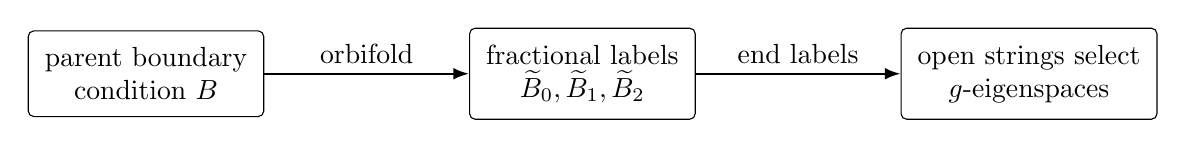
\begin{tikzpicture}[
  node distance=2.6cm,
  box/.style={draw, rounded corners=2pt, align=center, inner sep=6pt},
  arrow/.style={-{Latex[length=2mm]}, thick}
]
\node[box] (parent) {parent boundary\\condition $B$};
\node[box, right=of parent] (frac) {fractional labels\\$\wt B_0,\wt B_1,\wt B_2$};
\node[box, right=of frac] (open) {open strings select\\$g$-eigenspaces};
\draw[arrow] (parent) -- node[above]{orbifold} (frac);
\draw[arrow] (frac) -- node[above]{end labels} (open);
\end{tikzpicture}
\caption{Fractional branes are boundary conditions in the orbifold CFT. Their labels determine
which eigenspace of the parent open-string Hilbert space appears. The drawing suppresses
oscillator content and only shows the bookkeeping map from boundary labels to projections.}
\label{fig:fractional-bookkeeping}
\end{figure}

\subsection{Fractional ED3 and Fractional D7 Labels}

Let $\wt I_a$ denote the fractional ED3 instanton boundary condition, with
$a\in\{0,1,2\}$. Let $\wt S_m$ denote a fractional space-filling D7 boundary condition, with
$m\in\{0,1,2\}$. The notation $S$ stands for ``space-filling'' in $\R^{1,3}$; it does not
mean that the internal boundary condition is the same as that of the instanton.

For an oriented string from the instanton to a space-filling brane, define
\begin{equation}
  \cH_{a m}^{I S}
  :=
  \cH_{\wt I_a\wt S_m}.
\end{equation}
If the parent internal boundary conditions are $I$ and $S$, then
\begin{equation}
  \cH_{a m}^{I S}
  \simeq
  \left(\cH_{I S}\right)_{\omega^{a-m}}.
  \label{eq:IS-eigenspace}
\end{equation}
The reverse orientation uses the conjugate eigenspace
$\left(\cH_{S I}\right)_{\omega^{m-a}}$.

\section{Orientifold Involutions}

An orientifold action is a worldsheet orientation reversal combined with a target-space
involution. For the O7 orientifold used below we write it as
\begin{equation}
  \orient = (-1)^{F_L}\Omega \circ \sigma .
  \label{eq:orientifold-convention}
\end{equation}
Here $\Omega$ reverses the worldsheet orientation, $F_L$ is the left-moving spacetime fermion
number, and $\sigma$ acts on the target space. Omitting $(-1)^{F_L}$ would define a different
orientifold with different RR crosscap signs, so the coefficients $C_\ell$ below would have to
be recomputed.

The orientifold also acts on fractional labels. In a lift for which
\begin{equation}
  \orient\,|B,g^\ell\rangle=\kappa_\ell\,|B,g^{-\ell}\rangle,
  \qquad
  \kappa_\ell\in U(1),
  \label{eq:orientifold-twisted-lift}
\end{equation}
one has
\begin{equation}
  \orient\,|\wt B_m\rangle
  =
  \frac{1}{\sqrt{3}}\sum_{\ell=0}^2
  \omega^{m\ell}\kappa_\ell\,|B,g^{-\ell}\rangle.
  \label{eq:orientifold-label-general}
\end{equation}
For the minimal lift $\kappa_\ell=1$, this gives
\begin{equation}
  \orient\,|\wt B_m\rangle=|\wt B_{-m}\rangle.
  \label{eq:orientifold-label-minimal}
\end{equation}
Thus label $0$ can support a single invariant O(1) instanton, while labels $1$ and $2$ are
exchanged and require an invariant linear combination. A nontrivial lift $\kappa_\ell$ changes
this label map and is part of the crosscap data.

A common restricted class of lifts multiplies the minimal lift by a quantum-symmetry character,
\begin{equation}
  \kappa_\ell=\omega^{s\ell},
  \qquad
  s\in\{0,1,2\}.
  \label{eq:character-lift}
\end{equation}
Then
\begin{equation}
  \orient\,|\wt B_m\rangle=|\wt B_{s-m}\rangle.
  \label{eq:orientifold-label-character}
\end{equation}
An invariant one-node O(1) instanton must obey $2a=s\pmod 3$. Thus, after the bootstrap fixes
the lift $s$, the invariant label is $a=2s\pmod 3$. This lift must be fixed before computing
the ED3-D7 zero-mode spectrum.

For later use, the three character lifts are:
\begin{center}
\begin{tabular}{@{}llll@{}}
\toprule
lift $s$ & label map & one-node invariant label & D7-image constraint \\
\midrule
$0$ & $m\mapsto -m$ & $a=0$ & $N_1=N_2$ \\
$1$ & $m\mapsto 1-m$ & $a=2$ & $N_0=N_1$ \\
$2$ & $m\mapsto 2-m$ & $a=1$ & $N_0=N_2$ \\
\bottomrule
\end{tabular}
\end{center}
Here $N_m$ is the D7 boundary-state coefficient defined in
\eqref{eq:D7-boundary-vector}. These equalities only identify orientifold images. They do not
replace the RR tadpole equations.

\subsection{O7 Involution on the Exceptional Divisor}

The involution used in the \(K_0\) computation is
\begin{equation}
  \sigma_1 : [z_1,z_2,z_3;p]\longmapsto [z_1,z_2,z_3;-p].
  \label{eq:sigma1}
\end{equation}
Its fixed locus is $E=\{p=0\}\simeq \CP^2$, so it produces an O7-plane wrapping the
exceptional divisor. On the $\C^3$ cover of the orbifold point the same involution is represented
by
\begin{equation}
  R:(Z^1,Z^2,Z^3)\longmapsto (-Z^1,-Z^2,-Z^3).
  \label{eq:sigma1-cover-lift}
\end{equation}
Indeed, the projective equivalence
\((z_1,z_2,z_3;p)\sim(-z_1,-z_2,-z_3;-p)\) is the special case
\(\lambda=-1\) of \eqref{eq:projective-relation}. Thus \(\sigma_1\) is trivial on the
homogeneous base point \([z_1,z_2,z_3]\), but it is not trivial on the cover fields whose
oscillators enter the orbifold BCFT. In an open-channel twined trace the oscillator phase
associated with \(R g^\ell\) is therefore \(-\omega^\ell\) on \(Z^i\) and
\(-\omega^{-\ell}\) on \(\bar Z^{\bar i}\). The discrete datum still to specify is the lift of this
geometric action to the fractional Chan--Paton and spin structures; that lift is fixed by the
unoriented modular bootstrap.

\section{O(1) Instanton Convention and Universal Zero Modes}

\begin{assumption}[O(1) projection]
The fractional ED3 instanton is invariant under the orientifold, possibly after identifying it
with its image fractional label. Its Chan-Paton projection is fixed so that the four
translation modes in $\R^{1,3}$ survive and the unwanted gauge ghost zero modes are projected
out. This is the O(1) instanton convention.
\end{assumption}

Under this assumption the universal zero modes are:
\begin{itemize}
\item four bosonic zero modes $x^\mu$, $\mu=0,1,2,3$, for translations in $\R^{1,3}$;
\item two fermionic zero modes $\theta^\alpha$, $\alpha=1,2$, associated with the two
supercharges broken by the O(1) instanton.
\end{itemize}
The absence of additional ED3 deformation modes is a rigidity assumption about the fractional
instanton boundary condition. If extra neutral or charged zero modes appear in the fractional
open-string spectrum, the standalone \(K_0\) formula used in this note is not the applicable
object.

\section{RR Tadpoles and the Crosscap Vector}

Let $N_m$ be the total boundary-state coefficient of fractional D7-branes of label $m$ in the
orientifold theory. Thus $N_m$ counts the branes and images that actually couple to RR fields in
the quotient convention used for the annulus formula; it is not an additional covering-space
multiplicity. The total D7 boundary state is
\begin{equation}
  |S\rangle_{\RR}
  =
  \sum_{m=0}^{2}N_m|\wt S_m\rangle_{\RR}
  =
  \frac{1}{\sqrt{3}}\sum_{\ell=0}^{2}
  \left(\sum_{m=0}^{2}N_m\omega^{m\ell}\right)
  |S,g^\ell\rangle_{\RR}.
  \label{eq:D7-boundary-vector}
\end{equation}
Let the RR crosscap state be written as
\begin{equation}
  |C\rangle_{\RR}
  =
  \sum_{\ell=0}^{2}C_\ell\,|C,g^\ell\rangle_{\RR},
  \label{eq:crosscap-vector}
\end{equation}
where $C_\ell$ are crosscap coefficients. The symbols $|S,g^\ell\rangle_{\RR}$ and
$|C,g^\ell\rangle_{\RR}$ denote RR Ishibashi-state components in the $g^\ell$ sector; their
normalization must be fixed before comparing $C_\ell$ with the D7 coefficients.

The local RR tadpole cancellation condition is the sector-by-sector equation
\begin{equation}
  \frac{1}{\sqrt{3}}\sum_{m=0}^{2}N_m\omega^{m\ell}
  + C_\ell =0,
  \qquad
  \ell=0,1,2,
  \label{eq:tadpole-vector}
\end{equation}
after all states are expressed in the same Ishibashi basis.

Equivalently, once the crosscap coefficients $C_\ell$ are known in this basis, the D7 vector is
fixed by the inverse discrete Fourier transform
\begin{equation}
  N_m
  =
  -\frac{1}{\sqrt{3}}\sum_{\ell=0}^{2} C_\ell\,\omega^{-m\ell},
  \qquad
  m=0,1,2.
  \label{eq:tadpole-inverse}
\end{equation}
This formula is exact in the stated boundary-state normalization. A proposed crosscap vector is
therefore admissible only if the right hand side gives nonnegative integers compatible with the
orientifold image constraints for the lift $s$.

\begin{assumption}[Symmetric D7 distribution]
When the crosscap has no uncancelled twisted RR charge in the stated normalization, a symmetric
distribution
\begin{equation}
  N_0=N_1=N_2=N
  \label{eq:symmetric-D7}
\end{equation}
cancels the boundary contribution in the $\ell=1,2$ twisted sectors because
$1+\omega+\omega^2=0$. If the untwisted O7 charge is $-8$ in bulk D7 units, then in the
normalization of \eqref{eq:tadpole-vector} this means $C_0=-8\sqrt{3}$ and $N=8$ gives
24 fractional D7 boundary-state units, corresponding to 8 bulk D7-branes.
\end{assumption}

The symmetric D7 assumption is not a replacement for a crosscap computation. If $C_1$ or
$C_2$ is nonzero, then the D7 multiplicities must solve the full vector equation
\eqref{eq:tadpole-vector}.

\subsection{Crosscap Vector from Factorization}

The coefficients $C_\ell$ are fixed by factorizing unoriented one-loop diagrams into the
closed-string channel.

Let
\begin{equation}
  B_m^\ell=\frac{\omega^{m\ell}}{\sqrt{3}},
  \qquad
  Q_S^\ell=\sum_{m=0}^{2}N_m B_m^\ell
  =
  \frac{1}{\sqrt{3}}\sum_{m=0}^{2}N_m\omega^{m\ell}.
  \label{eq:D7-sector-charge}
\end{equation}
Here $B_m^\ell$ is the coefficient of the RR Ishibashi block labelled by $g^\ell$ in the
fractional D7 boundary state $\wt S_m$, and $Q_S^\ell$ is the total D7 charge coefficient in
that block. In the notation of \eqref{eq:tadpole-vector}, $Q_S^\ell$ is the first term.

The following equations display only the coefficient of a fixed massless RR Ishibashi block.
The common closed-string propagator, ghost insertion, and oscillator character in that block are
denoted by $\mathcal I_\ell(\ell_c)$, where $\ell_c$ is the closed-channel Schwinger parameter.
Thus no oscillator or normalization factor is being silently discarded; all such factors are
contained in the same object $\mathcal I_\ell$ on the annulus, Mobius, and Klein bottle sides.
With this convention, the RR tadpole part of the tree-channel D7 annulus, D7 Mobius strip, and
Klein bottle has the form
\begin{align}
  \widetilde{\mathcal A}_{SS}^{\RR}
  &=
  \sum_{\ell=0}^{2} Q_S^\ell Q_S^{-\ell}\,\mathcal I_\ell,
  \label{eq:tree-annulus-SS}
  \\
  \widetilde{\mathcal M}_{S}^{\RR}
  &=
  2\sum_{\ell=0}^{2} Q_S^\ell C_{-\ell}\,\mathcal I_\ell,
  \label{eq:tree-mobius-S}
  \\
  \widetilde{\mathcal K}^{\RR}
  &=
  \sum_{\ell=0}^{2} C_\ell C_{-\ell}\,\mathcal I_\ell.
  \label{eq:tree-klein}
\end{align}
The tilde means that the expression has been modular transformed to the closed-string channel.
For real D7 multiplicities, $Q_S^{-\ell}=(Q_S^\ell)^*$. A consistent crosscap has the analogous
reality condition $C_{-\ell}=C_\ell^*$ in a conjugation-compatible Ishibashi basis. Therefore the
sum of the three tree-channel RR tadpole contributions factorizes as
\begin{equation}
  \widetilde{\mathcal A}_{SS}^{\RR}
  +\widetilde{\mathcal M}_{S}^{\RR}
  +\widetilde{\mathcal K}^{\RR}
  =
  \sum_{\ell=0}^{2}
  \left(Q_S^\ell+C_\ell\right)
  \left(Q_S^{-\ell}+C_{-\ell}\right)
  \mathcal I_\ell.
  \label{eq:tadpole-factorization}
\end{equation}
Equation \eqref{eq:tadpole-vector} is exactly the condition that each factor
$Q_S^\ell+C_\ell$ vanishes.

In practice the crosscap vector is obtained in two stages.
First, compute the direct-channel Klein bottle trace with orientifold insertions
\begin{equation}
  \mathcal K^{\RR}(t)
  =
  \frac{1}{2\cdot 3}
  \sum_{r=0}^{2}
  \operatorname{Tr}_{\cH_{\rm closed}^{\RR}}
  \left(
    \orient\, g^r\,P_{\rm GSO}^{\rm closed}\,
    \e^{-2\pi t(L_0+\bar L_0-c/12)}
  \right),
  \label{eq:direct-klein-trace}
\end{equation}
where $P_{\rm GSO}^{\rm closed}$ is the closed-string GSO projector and $c$ is the total
worldsheet central charge of the traced sector. After the appropriate Klein-bottle modular
transformation, \eqref{eq:direct-klein-trace} fixes the products $C_\ell C_{-\ell}$ in
\eqref{eq:tree-klein}. This fixes magnitudes and relative support in twisted sectors, but by
itself it may not fix all phases of $C_\ell$.

Second, compute a Mobius amplitude with a probe fractional D7 boundary state whose coefficients
$B_m^\ell$ are already known from \eqref{eq:D7-sector-charge}. In the closed channel it must have
the coefficient structure
\begin{equation}
  \widetilde{\mathcal M}_{m}^{\RR}
  =
  2\sum_{\ell=0}^{2} B_m^\ell C_{-\ell}\,\mathcal I_\ell.
  \label{eq:probe-mobius-factorization}
\end{equation}
This comparison fixes the phases of $C_\ell$ relative to the fractional D7 boundary-state basis
and also fixes the lift phases $\kappa_\ell$ in \eqref{eq:orientifold-twisted-lift}. This is the
step hidden by the informal phrase ``O7 charge multiplier'' in rough calculations. The O7 charge
is a closed-channel crosscap coefficient; it is not a scalar multiplying the open-channel Mobius
character.

There are three useful consistency checks on the result. First,
\begin{equation}
  C_{-\ell}=C_\ell^*
  \label{eq:crosscap-reality}
\end{equation}
in a basis where the $g^\ell$ and $g^{-\ell}$ Ishibashi blocks are conjugate. Second, the inverse
transform \eqref{eq:tadpole-inverse} must give nonnegative integers $N_m$. Third, for a character
lift $m\mapsto s-m$, the solution must obey the image constraint $N_m=N_{s-m}$.

\begin{proposition}[Untwisted charge already forces local D7 charge]
Assume that the D7 multiplicities obtained from \eqref{eq:tadpole-inverse} are nonnegative
integers. Then
\begin{equation}
  \sum_{m=0}^{2}N_m=-\sqrt{3}\,C_0.
  \label{eq:total-D7-from-C0}
\end{equation}
In particular, if the involution-I O7$^-$ crosscap has $C_0=-8\sqrt{3}$ in the normalization of
\eqref{eq:tadpole-vector}, then every tadpole solution has total local D7 multiplicity
\begin{equation}
  \sum_{m=0}^{2}N_m=24.
  \label{eq:total-D7-o7minus}
\end{equation}
\end{proposition}

\begin{proof}
Sum \eqref{eq:tadpole-inverse} over $m$. Since
$\sum_{m=0}^{2}\omega^{-m\ell}=3\delta_{\ell,0}$, only the untwisted coefficient $C_0$ remains.
\end{proof}

The consequence for a one-node invariant instanton is stated precisely in
Corollary~\ref{cor:pureK0-obstructed-by-untwisted-charge}, after the local ED3-D7 zero-mode
test has been derived.

\section{Theta Functions and Characters}

We use the theta-function convention
\begin{equation}
  q=\e^{2\pi \ii\tau},
  \qquad
  \vart_{\alpha\beta}(\tau)
  =
  \sum_{n\in\Z}
  (-1)^{\beta n}
  q^{(n+\alpha/2)^2/2},
  \qquad
  \alpha,\beta\in\{0,1\}.
  \label{eq:theta-convention}
\end{equation}
Thus $\vart_{00}$, $\vart_{01}$, and $\vart_{10}$ are the usual $\theta_3$, $\theta_4$,
and $\theta_2$ at zero argument, while $\vart_{11}(\tau)=0$. When a characteristic such as
$\alpha+Q$ appears below, it is reduced modulo $2$ with this convention. The Dedekind eta
function is
\begin{equation}
  \etaD(\tau)=q^{1/24}\prod_{n=1}^{\infty}(1-q^n).
  \label{eq:dedekind-eta-definition}
\end{equation}

The internal Calabi-Yau SCFT has central charge $c=9$ and an extended
$\mathcal N=2$ superconformal algebra. Massive representations are labelled by
$(h,Q)$, where $h$ is the conformal weight and $Q\in\{0,1\}$ is the charge label used in the
extended-character convention. For a massive representation, the character components are
\begin{equation}
  g_{\alpha\beta}^{(h,Q)}(\tau)
  =
  (-1)^{\beta Q}
  \frac{q^{h-(1+Q)/4}}{\etaD(\tau)^3}
  \vart_{\alpha\beta}(\tau)
  \vart_{\alpha+Q,0}(2\tau).
  \label{eq:massive-character}
\end{equation}
Massless representations are denoted $(\vac)$, $(+)$, and $(-)$. The vacuum representation
contains the $SL(2,\R)$ invariant vacuum.

\section{Annulus Contributions}

In this section \(Z_{A,\DD}\) means the annulus with both boundaries on the fractional ED3, and
\(Z_{A,\DN}\) means the annulus with one boundary on the ED3 and one boundary on the D7 stack.
The letters \(\DD\) and \(\DN\) refer to the four non-compact spacetime directions; the internal
\(\C^3/\Z_3\) data are carried by the fractional labels and character multiplicities.

\subsection{Both Boundaries on the Fractional Instanton}

Let $Z_{A,\DD}$ be the annulus contribution with both boundaries on the fractional instanton.
For each representation of the extended $\mathcal N=2$ algebra, the universal free-field
identity gives
\begin{equation}
  Z_{A,\DD}^{(r)}=0.
  \label{eq:DD-vanishing}
\end{equation}
This is exact under the assumptions of the reference: no additional zero modes beyond the
universal O(1) modes and a boundary condition preserving the relevant extended algebra. The
identity is not a statement that the instanton has no zero modes; it is a statement about the
massive non-zero-mode annulus contribution after the supersymmetric spin-structure sum.

\subsection{One Boundary on the Instanton and One on a Space-filling Brane}

The universal open-string block imported from the D-instanton reference is the block in which
the four non-compact fields $X^\mu,\psi^\mu$ have mixed Dirichlet-Neumann boundary
conditions. The instanton is Dirichlet in $\R^{1,3}$ and the D7-brane is Neumann in
$\R^{1,3}$. The internal fractional CFT data are not replaced by a six-dimensional DN free
field block; they enter through signed coefficients of extended $\mathcal N=2$ characters.

In the reference convention, the contribution of a massive representation $(h,Q)$ is
\begin{equation}
  Z_{A,\DN}^{(h,Q)}
  =
  \frac{(-1)^Q}{2}\,
  q^{h-(1+Q)/4}\,
  \vart_{1-Q,0}(2\tau).
  \label{eq:universal-DN-block}
\end{equation}
After summing over representations, the annulus has the form
\begin{equation}
  Z_{A,\DN}(\tau)
  =
  \sum_{Q=0}^{1}
  \frac{(-1)^Q}{2}\,
  \vart_{1-Q,0}(2\tau)
  \sum_{h\ge |Q|/2}
  n_{h,Q}\,
  q^{h-(1+Q)/4}.
  \label{eq:DN-annulus}
\end{equation}
Here $n_{h,Q}$ is the signed coefficient of representation $(h,Q)$ in the character expansion of
the open-string spectrum between the fractional instanton and the tadpole-cancelling
space-filling branes, in the same orientation convention as \eqref{eq:universal-DN-block}. For a
genuine massive representation this is an ordinary multiplicity. For massless representations it
can be signed; for example the vacuum representation contributes $+1$ to $(h,Q)=(0,0)$ and $-1$
to $(h,Q)=(1/2,1)$ in the massive-character basis used by the reference.

For a single fractional instanton $\wt I_a$ and D7 multiplicities $N_m$, this means
\begin{equation}
  n_{h,Q}
  =
  \sum_{m=0}^{2} N_m\, n_{h,Q}^{(a,m)},
  \label{eq:multiplicity-sum}
\end{equation}
where $n_{h,Q}^{(a,m)}$ is computed from the eigenspace
$\cH_{a m}^{I S}$ in \eqref{eq:IS-eigenspace}. This is linear in the D7 multiplicities because
one boundary is the single O(1) instanton. If there are $k_a$ identical instantons of label
$a$, the right hand side is multiplied by $k_a$ before the multi-instanton zero-mode analysis.

Equivalently, let $\mathcal R_{h,Q}^{I S}$ be the multiplicity space of the representation
$(h,Q)$ in the parent internal open-string Hilbert space $\cH_{I S}$, with signed character
decomposition understood as above. Then the fractional projection gives the exact coefficient
\begin{equation}
  n_{h,Q}^{(a,m)}
  =
  \frac{1}{3}
  \sum_{\ell=0}^{2}
  \omega^{-(a-m)\ell}\,
  \Tr_{\mathcal R_{h,Q}^{I S}}\!\left(g^\ell\right).
  \label{eq:DN-projection-coefficient}
\end{equation}
This formula is the corrected replacement for a double orbifold sum in the open channel. It
projects the parent internal spectrum onto the eigenspace selected by the two fractional labels.
It is written for the ordered sector $I\to S$. The reverse orientation is the ordered sector
$S\to I$ and has
\begin{equation}
  n_{h,Q}^{(m,a);S I}
  =
  \frac{1}{3}
  \sum_{\ell=0}^{2}
  \omega^{-(m-a)\ell}\,
  \Tr_{\mathcal R_{h,Q}^{S I}}\!\left(g^\ell\right).
  \label{eq:reverse-DN-projection}
\end{equation}
The APS block \eqref{eq:universal-DN-block} is normalized so that the two open-string
orientations are already paired when the two ordered sectors are related by charge conjugation.
Thus the reverse orientation is not a second D7 boundary label and should not be represented by a
second sum over D7 multiplicities.

\subsection{Twined Character Data and \texorpdfstring{$\Z_3$}{Z3} Charge Sectors}

The annulus data can be organized as a finite Fourier problem for each extended
\(\mathcal N=2\) representation. For a massive representation \((h,Q)\) in the parent ordered
\(I\to S\) internal Hilbert space, define the three twined traces
\begin{equation}
  T_{h,Q}^{IS}(\ell)
  =
  \Tr_{\mathcal R_{h,Q}^{IS}}\!\left(g^\ell\right),
  \qquad
  \ell=0,1,2,
  \label{eq:twined-massive-traces}
\end{equation}
where \(\mathcal R_{h,Q}^{IS}\) is the multiplicity space used in
\eqref{eq:DN-projection-coefficient}. The corresponding \(\Z_3\)-charge-sector multiplicities
are
\begin{equation}
  d_{h,Q;r}^{IS}
  =
  \frac{1}{3}\sum_{\ell=0}^{2}\omega^{-r\ell}T_{h,Q}^{IS}(\ell),
  \qquad
  r\in\Z/3\Z.
  \label{eq:charge-sector-multiplicities}
\end{equation}
Equivalently,
\begin{equation}
  T_{h,Q}^{IS}(\ell)
  =
  \sum_{r=0}^{2}d_{h,Q;r}^{IS}\omega^{r\ell}.
  \label{eq:inverse-charge-sector-transform}
\end{equation}
Here \(r\) is a worldsheet/orbifold eigenvalue label, not a transverse or spinor index. The
fractional boundary labels select one of these three charge sectors:
\begin{equation}
  n_{h,Q}^{(a,m)}
  =
  d_{h,Q;\,a-m}^{IS},
  \qquad
  a-m\ \text{read in}\ \Z/3\Z.
  \label{eq:fractional-coefficient-charge-sector}
\end{equation}
Equation \eqref{eq:fractional-coefficient-charge-sector} is just
\eqref{eq:DN-projection-coefficient} rewritten after the finite Fourier transform
\eqref{eq:charge-sector-multiplicities}. Thus the missing massive annulus data are precisely
the integers \(d_{h,Q;r}^{IS}\), representation by representation.

For the symmetric tadpole solution \(N_0=N_1=N_2=8\), the total DN coefficient for a single
instanton label \(a\) simplifies to the untwined parent multiplicity:
\begin{equation}
  n_{h,Q}^{(a)}
  =
  \sum_{m=0}^2 N_m n_{h,Q}^{(a,m)}
  =
  8\sum_{r=0}^{2}d_{h,Q;r}^{IS}
  =
  8\,T_{h,Q}^{IS}(0).
  \label{eq:symmetric-annulus-untwined-parent}
\end{equation}
This simplification applies to the non-zero-mode determinant once the zero-mode rows have been
handled separately. It does not mean that the charged zero modes vanish; it only says that equal
fractional D7 multiplicities remove the phase dependence from the total annulus coefficient.

The low-lying data already fixed in this note are the massless row analogues of
\eqref{eq:twined-massive-traces}:
\begin{equation}
  T_{\vac}^{IS}(\ell)=1,
  \qquad
  T_{+}^{IS}(\ell)=3\omega^\ell,
  \qquad
  T_{-}^{IS}(\ell)=3\omega^{-\ell}.
  \label{eq:low-lying-twined-row-traces}
\end{equation}
Their charge-sector multiplicities are
\begin{equation}
  d_{\vac;r}^{IS}=\delta_{r,0},
  \qquad
  d_{+;r}^{IS}=3\delta_{r,1},
  \qquad
  d_{-;r}^{IS}=3\delta_{r,-1}.
  \label{eq:low-lying-charge-sector-multiplicities}
\end{equation}
Substituting \eqref{eq:low-lying-charge-sector-multiplicities} into
\eqref{eq:fractional-coefficient-charge-sector} reproduces the local zero-mode vector
\eqref{eq:local-zero-mode-vector}. The parent oscillator generating function in the next
subsection fills the same charge-sector table for the massive representations that remain in
\(Z_A^{\rm det}\), and the result resums to the \(A_2\)-theta formula in
\eqref{eq:DN-annulus-A2-closed-form}.

\subsection{Parent Oscillator Generating Function for the Twined Traces}

The Fourier transform above reduces the annulus data to the parent twined traces
\(T_{h,Q}^{IS}(\ell)\). This subsection records the raw free-field oscillator trace from which
those traces are extracted in the standard parent-boundary convention.

\begin{assumption}[Parent internal oscillator convention]
For the involution-I ED3-D7 system, the fractional ED3 and the local D7 stack are taken to have
the same internal parent boundary condition. Thus the internal ED3-D7 open string has no
additional internal DN directions: the only DN directions are the four non-compact spacetime
directions already accounted for in \eqref{eq:universal-DN-block}. In this boundary condition the parent
internal oscillator algebra is generated by three complex bosons \(Z^i\) and three complex
fermions \(\psi^i\), \(i=1,2,3\), with the orbifold action in \eqref{eq:z3-action} and
\eqref{eq:fermion-orbifold-action}. If a different D7 boundary condition is specified, the
generating function below must be replaced before computing \(K_0\).
\label{assumption:parent-oscillator-convention}
\end{assumption}

Let \(x\) be a formal variable that records the \(\Z_3\) eigenvalue, let \(u\) record the
internal \(U(1)\) charge, let \(s\) record worldsheet fermion parity, and let \(q\) record
oscillator energy above the NS open-string vacuum. The parent NS oscillators have the following
weights:
\begin{center}
\begin{tabular}{@{}lllll@{}}
\toprule
oscillator & range & oscillator energy & \(x\)-weight & \(u\)-weight \\
\midrule
\(\alpha^i_{-n}\) & \(n\ge 1\) & \(n\) & \(x\) & \(1\) \\
\(\bar\alpha^{\bar i}_{-n}\) & \(n\ge 1\) & \(n\) & \(x^{-1}\) & \(1\) \\
\(\psi^i_{-r}\) & \(r\in \Z_{\ge0}+\frac12\) & \(r\) & \(x\) & \(u\) \\
\(\bar\psi^{\bar i}_{-r}\) & \(r\in \Z_{\ge0}+\frac12\) & \(r\) & \(x^{-1}\) & \(u^{-1}\) \\
\bottomrule
\end{tabular}
\end{center}
The index \(i\) or \(\bar i\) runs over \(1,2,3\). The variables \(x,u,s\) are bookkeeping
variables only: \(x\) is reduced to \(x=\omega^\ell\) when a twined trace is evaluated, \(u\)
is used to decompose into internal \(U(1)\)-charge sectors, and \(s=-1\) inserts
\((-1)^f\) in the NS oscillator trace.

The corresponding raw NS generating function is
\begin{equation}
  \mathcal P_{\NS}(x,u,s;q)
  =
  \prod_{n=1}^{\infty}
  \frac{1}
  {(1-xq^n)^3(1-x^{-1}q^n)^3}
  \prod_{r\in\Z_{\ge0}+\frac12}
  (1+suxq^r)^3(1+su^{-1}x^{-1}q^r)^3 .
  \label{eq:parent-NS-oscillator-generating-function}
\end{equation}
This is the parent oscillator trace before the Chan-Paton fractional projection, the GSO
projection, the orientifold projection, and the subtraction of charged zero-mode
representatives. The physical annulus coefficient is obtained only after these four operations
are applied.

If \(\epsilon_{\NS}=+1\) keeps NS states with even worldsheet fermion parity and
\(\epsilon_{\NS}=-1\) keeps NS states with odd worldsheet fermion parity, the NS GSO-projected
raw trace in this convention is
\begin{equation}
  \mathcal P_{\NS}^{(\epsilon_{\NS})}(x,u;q)
  =
  \frac12\left[
    \mathcal P_{\NS}(x,u,+1;q)
    +
    \epsilon_{\NS}\mathcal P_{\NS}(x,u,-1;q)
  \right].
  \label{eq:parent-NS-GSO-ledger}
\end{equation}
The sign \(\epsilon_{\NS}\) is not determined by \eqref{eq:parent-NS-GSO-ledger}; it must agree
with the open-string GSO projection used in the BCFT zero-mode projection. With this GSO
projection fixed,
the raw NS multiplicity at
oscillator energy \(E\), internal charge \(J\), and \(\Z_3\) charge \(r\) is
\begin{equation}
  p_{\NS}^{(\epsilon_{\NS})}(E,J;r)
  =
  \frac13\sum_{\ell=0}^2
  \omega^{-r\ell}\,
  [q^E u^J]\,
  \mathcal P_{\NS}^{(\epsilon_{\NS})}(\omega^\ell,u;q),
  \label{eq:raw-NS-charge-sector-ledger}
\end{equation}
where \([q^E u^J]\) means ``coefficient of \(q^E u^J\).'' This formula is a finite
\(\Z_3\) Fourier projection of the parent oscillator trace. It should not be confused with
\(d_{h,Q;r}^{IS}\) in \eqref{eq:charge-sector-multiplicities}: \(p_{\NS}\) counts raw
oscillator states, while \(d_{h,Q;r}^{IS}\) counts multiplicity spaces of extended
\(\mathcal N=2\) representations after the character decomposition.

The character extraction is triangular in the \(q\)-expansion. In the stated normalization of
the internal NS characters, write
\begin{equation}
  \mathcal P_{\NS}^{(\epsilon_{\NS})}(\omega^\ell,u;q)
  =
  \sum_{\lambda\in\{\vac,+,-\}}
  A_{\lambda}^{IS}(\ell)\,\chi_{\lambda,\NS}(u;q)
  +
  \sum_{(h,Q)}
  T_{h,Q}^{IS}(\ell)\,\chi_{h,Q,\NS}(u;q).
  \label{eq:NS-character-extraction}
\end{equation}
Here \(\chi_{\lambda,\NS}\) is the NS character of the massless internal representation
\(\lambda\in\{\vac,+,-\}\), \(\chi_{h,Q,\NS}\) is the NS character of the massive
representation labelled by \((h,Q)\), and \(A_{\lambda}^{IS}(\ell)\) are the twined
coefficients of the three massless rows. The massive coefficients in
\eqref{eq:NS-character-extraction} are precisely the traces \(T_{h,Q}^{IS}(\ell)\) used in
\eqref{eq:twined-massive-traces}. The extraction is triangular because each character has a
definite lowest power of \(q\); after subtracting all characters that begin below a given
power, the coefficient at the next lowest power fixes the next multiplicity.

As a check on the normalization, the first terms of the raw NS generating function are
\begin{equation}
  \mathcal P_{\NS}(x,u,s;q)
  =
  1
  +
  3sux\,q^{1/2}
  +
  3su^{-1}x^{-1}q^{1/2}
  +
  \left[
    3(x+x^{-1})
    +
    9
    +
    3u^2x^2
    +
    3u^{-2}x^{-2}
  \right]q
  +
  O(q^{3/2}).
  \label{eq:parent-NS-first-terms}
\end{equation}
Setting \(x=\omega^\ell\) reproduces the low-lying twined row traces in
\eqref{eq:low-lying-twined-row-traces}. Thus the oscillator trace and the local row analysis
use the same \(\Z_3\)-charge convention. The \(q\)-order terms are displayed to make the next
step concrete: they are raw oscillator states with \((J,r)=(0,1),(0,-1),(0,0),(2,-1)\), and
\((-2,1)\), respectively, where \(J\) is the internal \(U(1)\) charge and \(r\) is the
\(\Z_3\) charge. They are not representation multiplicities: descendants of the massless
characters in \eqref{eq:NS-character-extraction} must first be subtracted.

\subsection{Ramond Ground States and the Spin Lift}

The Ramond sector requires one more piece of local BCFT data: the lift of the orbifold
generator \(g\) to spin fields. This lift is easy to miss because \(g\) has order three on
vectors but its naive spin representative has order six.

Bosonize the three complex internal fermions by
\begin{equation}
  \psi^i=\e^{\ii H_i},
  \qquad
  \bar\psi^{\bar i}=\e^{-\ii H_i},
  \qquad
  i=1,2,3.
  \label{eq:fermion-bosonization}
\end{equation}
The Ramond ground states are spin fields
\begin{equation}
  S_{\varepsilon}
  =
  \exp\left[
    \frac{\ii}{2}\sum_{i=1}^3 \varepsilon_i H_i
  \right],
  \qquad
  \varepsilon_i=\pm 1.
  \label{eq:internal-spin-fields}
\end{equation}
Define
\begin{equation}
  J(\varepsilon)=\frac12\sum_{i=1}^3\varepsilon_i,
  \qquad
  n_-(\varepsilon)=\#\{i:\varepsilon_i=-1\}.
  \label{eq:spin-field-J-and-nminus}
\end{equation}
Here \(J(\varepsilon)=3/2-n_-(\varepsilon)\) is the internal \(U(1)\) charge of the spin field.
The vector action \(\psi^i\mapsto\omega\psi^i\) is represented on bosons by
\(H_i\mapsto H_i+2\pi/3\). The naive spin-field phase is therefore
\(\exp(2\pi\ii J(\varepsilon)/3)\), whose cube is \(-1\) on every spin field. To obtain an
order-three action on the Ramond ground states, multiply this naive lift by a phase
\(-\omega^\rho\), with
\begin{equation}
  \rho\in\Z/3\Z.
  \label{eq:spin-lift-rho}
\end{equation}
The resulting spin lift is
\begin{equation}
  g_R^{(\rho)}\,S_{\varepsilon}
  =
  \omega^{\,r_\rho(\varepsilon)}S_{\varepsilon},
  \qquad
  r_\rho(\varepsilon)=\rho-n_-(\varepsilon)\pmod 3.
  \label{eq:R-spin-lift-action}
\end{equation}
The parameter \(\rho\) is not a transverse index. It is a discrete spin-lift datum to be fixed
together with the closed-string GSO projection and the orientifold lift. The common
Calabi-Yau lift is \(\rho=0\), for which the two \(SU(3)\)-singlet spin fields with
\(n_-=0\) and \(n_-=3\) have \(\Z_3\) charge zero. The note does not assume this choice unless
it is stated explicitly.

The Ramond ground-state charge polynomial in this convention is
\begin{equation}
  \mathcal G_R^{(\rho)}(x,u)
  =
  x^\rho\bigl(u^{3/2}+u^{-3/2}\bigr)
  +
  3x^{\rho-1}u^{1/2}
  +
  3x^{\rho-2}u^{-1/2},
  \label{eq:R-ground-state-polynomial}
\end{equation}
where powers of \(x\) are read modulo \(3\) after setting \(x=\omega^\ell\). Equivalently, the
Ramond ground-state charge-sector multiplicities are
\begin{equation}
  \begin{array}{c|c|c|c}
  n_-(\varepsilon) & J(\varepsilon) & \text{multiplicity} & \Z_3\text{ charge }r \\
  \hline
  0 & 3/2 & 1 & \rho \\
  1 & 1/2 & 3 & \rho-1 \\
  2 & -1/2 & 3 & \rho-2 \\
  3 & -3/2 & 1 & \rho
  \end{array}
  \label{eq:R-ground-state-charge-table}
\end{equation}
all charges being in \(\Z/3\Z\). For a fractional ED3 of label \(a\) and a D7 label \(m\), the
orbifold projection keeps the row \(r=a-m\). Thus the raw Ramond ground states in
\(\cH^{IS}_{a m}\) are selected by
\begin{equation}
  m=a-r_\rho(\varepsilon)\pmod 3.
  \label{eq:R-ground-state-fractional-selection}
\end{equation}

After fixing the R-sector GSO parity \(\chi_R\), it is useful to record only the spin fields
that survive that parity. Define
\begin{equation}
  s_{\rho,\chi_R}(r)
  =
  \#\left\{
    \varepsilon\,\middle|\,
    n_-(\varepsilon)\equiv\chi_R\!\!\pmod2,\quad
    r_\rho(\varepsilon)=r
  \right\},
  \qquad r\in\Z/3\Z .
  \label{eq:R-spin-charge-multiplicity-definition}
\end{equation}
Here \(s_{\rho,\chi_R}(r)\) is a multiplicity of internal Ramond spin fields. The corresponding
fermionic \(L_0=0\) vertex dimension is obtained only after imposing the orientifold action and
the external vertex factors. The charge table
\eqref{eq:R-ground-state-charge-table} gives
\begin{equation}
  \begin{array}{c|ccc}
  & s_{\rho,\chi_R}(\rho) & s_{\rho,\chi_R}(\rho-1) & s_{\rho,\chi_R}(\rho-2) \\
  \hline
  \chi_R=0 & 1 & 0 & 3 \\
  \chi_R=1 & 1 & 3 & 0
  \end{array}
  \label{eq:R-spin-charge-multiplicity-table}
\end{equation}
with the three charge labels read modulo \(3\). Equivalently, for the common Calabi-Yau spin lift
\(\rho=0\),
\begin{equation}
  \begin{array}{c|ccc}
  & r=0 & r=1 & r=2 \\
  \hline
  \chi_R=0 & 1 & 3 & 0 \\
  \chi_R=1 & 1 & 0 & 3
  \end{array}
  \label{eq:R-spin-charge-multiplicity-rho-zero}
\end{equation}
This last display is only the \(\rho=0\) specialization; the formulas above keep \(\rho\)
explicit.

The same table gives a useful orientifold compatibility test. Suppose the R-sector orientifold
maps the source branch \((\rho,\chi_R)\) in the ordered \(I\to S\) sector to a target branch
\((\rho_\Theta,\chi_R^\Theta)\) in the ordered \(S\to I\) sector and conjugates the fractional
charge \(r\mapsto-r\). A finite invertible spin-field matrix can exist only if
\begin{equation}
  s_{\rho,\chi_R}(r)
  =
  s_{\rho_\Theta,\chi_R^\Theta}(-r),
  \qquad
  r=0,1,2.
  \label{eq:R-orientifold-branch-compatibility}
\end{equation}
Here \(-r\) is read in \(\Z/3\Z\). Comparing the two rows of
\eqref{eq:R-spin-charge-multiplicity-table} gives
\begin{equation}
  \rho_\Theta=-\rho\pmod3,
  \qquad
  \chi_R^\Theta=\chi_R+1\pmod2.
  \label{eq:R-orientifold-branch-map}
\end{equation}
Thus a charge-conjugating orientifold that acts with the same spin-lift label on source and target
forces \(\rho=0\), and it exchanges the two internal parity branches \(\chi_R=0\) and
\(\chi_R=1\). This is a statement about the internal Ramond spin fields only. If the full
open-string GSO projection packages the parity exchange with external or ghost factors, the
result must still satisfy \eqref{eq:R-orientifold-branch-compatibility}.

Equivalently, before the external DN spin fields, GSO projection, and orientifold projection
are imposed, the ordered \(I\to S\) Ramond ground-state shadows are
\begin{equation}
  W_{R,J}^{IS}(a;\rho)
  =
  \bigoplus_{\varepsilon:\,J(\varepsilon)=J}
  \C S_\varepsilon\otimes V_{a-r_\rho(\varepsilon)} .
  \label{eq:R-ground-state-ordered-spaces}
\end{equation}
Here \(V_m\) is the D7 Chan-Paton space of fractional label \(m\), with labels read modulo
\(3\). Their dimensions are
\begin{equation}
  \begin{array}{c|c}
  J & \dim W_{R,J}^{IS}(a;\rho) \\
  \hline
  3/2 & N_{a-\rho} \\
  1/2 & 3N_{a-\rho+1} \\
  -1/2 & 3N_{a-\rho+2} \\
  -3/2 & N_{a-\rho}
  \end{array}
  \label{eq:R-ground-state-local-vector}
\end{equation}
This is the Ramond analogue of the local vector \eqref{eq:local-zero-mode-vector}. It is a
ground-state multiplicity before the total open-string GSO projection, not a fermionic
zero-mode count. The two entries with \(J=\pm3/2\) are two internal spin-field rows; depending
on the external DN spin field and picture, one linear combination or chirality may be kept.

The nonzero Ramond oscillators have integer modes. Their oscillator generating function, before
the GSO and orientifold projections, is
\begin{equation}
  \mathcal P_R^{(\rho)}(x,u,s;q)
  =
  \mathcal G_R^{(\rho)}(x,u)
  \prod_{n=1}^{\infty}
  \frac{(1+suxq^n)^3(1+su^{-1}x^{-1}q^n)^3}
       {(1-xq^n)^3(1-x^{-1}q^n)^3}.
  \label{eq:parent-R-oscillator-generating-function}
\end{equation}
Here \(s\) records the parity of nonzero fermion oscillator excitations. The action of the full
open-string GSO operator on the Ramond ground states is not determined by
\eqref{eq:parent-R-oscillator-generating-function} alone, because it also involves the
non-compact DN spin fields and the specified picture. Consequently the R-sector charged
zero-mode spaces \(\mathcal B_{\lambda,R}^{\rm proj}(a)\) must still be evaluated as vertex
spaces, not inferred only from \(\mathcal G_R^{(\rho)}\).

The first nonzero-oscillator terms are
\begin{equation}
  \mathcal P_R^{(\rho)}(x,u,s;q)
  =
  \mathcal G_R^{(\rho)}(x,u)
  \left[
    1+
    3\left(x+x^{-1}+sux+su^{-1}x^{-1}\right)q
    +O(q^2)
  \right].
  \label{eq:parent-R-first-oscillator-terms}
\end{equation}
The terms \(3xq\) and \(3x^{-1}q\) come from the bosonic oscillators
\(\alpha^i_{-1}\) and \(\bar\alpha^{\bar i}_{-1}\), while the terms with \(s\) come from the
integer-moded R-sector fermion oscillators \(\psi^i_{-1}\) and
\(\bar\psi^{\bar i}_{-1}\). This is a raw oscillator expansion before the GSO projection and
before the Ramond vertex-space constraints.

For the symmetric tadpole solution \(N_0=N_1=N_2=8\), the dependence on \(a\) and \(\rho\) drops
out of the total raw Ramond ground-state count before the GSO and orientifold projections:
\begin{equation}
  \sum_{m=0}^2 N_m
  \sum_{\varepsilon:\,r_\rho(\varepsilon)=a-m}1
  =
  8\sum_{\varepsilon}1
  =
  64.
  \label{eq:symmetric-raw-R-ground-count}
\end{equation}
This number is only a raw internal spin-field count. It is not \(f_{\rm ch}\), not an annulus
coefficient, and not a determinant contribution until the external DN spin fields, GSO
projection, orientifold projection, and BRST vertex representatives have been included.

\subsection{External DN Boundary-changing Factors}

The internal generating functions above must be tensored with the universal four-dimensional DN boundary
changer. This subsection records that factor at the level needed for the zero-mode
calculation. It is local vertex data, not a global annulus formula.

Let \(\Delta_{IS}\) denote the bosonic boundary-changing operator that changes the four
non-compact coordinates \(X^\mu\), \(\mu=0,1,2,3\), from Dirichlet on the instanton boundary to
Neumann on the D7 boundary. Let \(\Delta_{SI}\) denote the reverse-orientation operator. For
four real DN bosons,
\begin{equation}
  h(\Delta_{IS})=h(\Delta_{SI})=\frac{4}{16}=\frac14.
  \label{eq:external-DN-bosonic-twist-weight}
\end{equation}
Here \(h\) is the holomorphic boundary conformal weight. The operator \(\Delta_{IS}\) has no
\(\Z_3\) charge because the orbifold acts only on the internal coordinates \(z_i\).

In the NS sector, the four DN fermions have zero modes. They generate a Clifford module for the
rotation group of the four non-compact DN directions. We denote the two states of one chirality
by
\begin{equation}
  S_{\DN}^{\mathsf s},
  \qquad
  \mathsf s=1,2,
  \qquad
  h(S_{\DN}^{\mathsf s})=\frac14.
  \label{eq:external-DN-NS-spin-fields}
\end{equation}
The index \(\mathsf s\) is an external DN spinor index, not an orbifold label and not an
internal \(SU(3)\) index. Which chirality is represented by \(S_{\DN}^{\mathsf s}\) is fixed by
the GSO branch; the opposite chirality is removed by \(P_{{\rm GSO},\NS}\).

Let \(\phi\) be the bosonized superghost, normalized so that
\begin{equation}
  h(\e^{-\phi})=\frac12,
  \qquad
  h(\e^{-\phi/2})=\frac38.
  \label{eq:superghost-weights}
\end{equation}
An ordered \(I\to S\) NS zero-mode vertex in the \((-1)\)-picture has the form
\begin{equation}
  V_{u}^{(-1)}
  =
  u_{\mathsf s,A}\,
  \Delta_{IS}\,
  S_{\DN}^{\mathsf s}\,
  \mathcal O_A^{\NS}\,
  \e^{-\phi},
  \label{eq:NS-charged-zero-mode-vertex-template}
\end{equation}
where \(u_{\mathsf s,A}\) is the coefficient of the zero-mode vertex and \(\mathcal O_A^{\NS}\) is an
internal boundary operator, including its Chan-Paton label. The condition that
\eqref{eq:NS-charged-zero-mode-vertex-template} have total boundary weight one is
\begin{equation}
  h(\mathcal O_A^{\NS})=0.
  \label{eq:NS-internal-zero-mode-weight}
\end{equation}
Thus, in the standard four-DN vertex construction, bosonic charged zero modes come from
internal NS operators of weight zero. Internal NS operators of higher weight can still enter the
massive annulus character expansion, but they are not \(L_0=0\) bosonic zero-mode vertices
of the form \eqref{eq:NS-charged-zero-mode-vertex-template}.

In the R sector, the DN fermions are half-integer moded and do not create an external spinor
zero-mode degeneracy. An ordered \(I\to S\) R zero-mode vertex in the \((-1/2)\)-picture has the
form
\begin{equation}
  V_{\eta}^{(-1/2)}
  =
  \eta_A\,
  \Delta_{IS}\,
  \mathcal S_A^{R}\,
  \e^{-\phi/2},
  \label{eq:R-charged-zero-mode-vertex-template}
\end{equation}
where \(\eta_A\) is the Grassmann coefficient of the zero-mode vertex and \(\mathcal S_A^{R}\) is an internal
Ramond boundary operator, including its Chan-Paton label. The weight-one condition is
\begin{equation}
  h(\mathcal S_A^{R})=\frac38.
  \label{eq:R-internal-zero-mode-weight}
\end{equation}
The internal spin fields \(S_\varepsilon\) in \eqref{eq:internal-spin-fields} have this weight.
Therefore the charge table \eqref{eq:R-ground-state-charge-table} is exactly the internal
Ramond ground-state input to the R-sector charged zero-mode calculation.

For later reference, the vertex-level zero-mode test can be split into a fixed kinematic part
and a projection part fixed by the GSO choice and orientifold lift:
\begin{equation}
  \begin{array}{c|c|c|c}
  \text{sector} & \text{external factor} & \text{internal weight required} &
  \text{projection still required} \\
  \hline
  \NS
  & \Delta_{IS}S_{\DN}^{\mathsf s}\e^{-\phi}
  & h_{\rm int}=0
  & P_{{\rm GSO},\NS},\ \Theta_{\NS} \\
  \mathrm R
  & \Delta_{IS}\e^{-\phi/2}
  & h_{\rm int}=3/8
  & P_{{\rm GSO},R},\ \Theta_R
  \end{array}
  \label{eq:external-DN-zero-mode-vertex-summary}
\end{equation}
Here \(\Theta_{\NS}\) and \(\Theta_R\) are the orientifold maps on the full vertex operators,
including the exchange \(\Delta_{IS}\leftrightarrow\Delta_{SI}\), the action on
\(S_{\DN}^{\mathsf s}\) in the NS sector, the internal action, and the Chan-Paton matrices.
These signs and matrices are not determined by the conformal weights in this subsection.

\subsection{Zero-mode Spaces After the DN Weight Test}

The vertex templates above refine the earlier row-level bookkeeping. Under
Assumption~\ref{assumption:parent-oscillator-convention}, the only internal NS operator of
weight zero is the identity row. Therefore the ordered \(I\to S\) NS charged zero-mode shadow is
\begin{equation}
  \mathcal Z_{\NS}^{IS}(a)
  =
  \C^2_{\DN,\NS}\otimes V_a,
  \qquad
  \dim \mathcal Z_{\NS}^{IS}(a)=2N_a.
  \label{eq:NS-zero-mode-space-after-DN-test}
\end{equation}
Here \(\C^2_{\DN,\NS}\) is spanned by the two external DN spin fields
\(S_{\DN}^{\mathsf s}\) that survive the fixed NS GSO chirality, and \(V_a\) is the D7
Chan-Paton space with the same fractional label as the instanton. The adjacent rows generated
by \(\psi^i\) and \(\bar\psi^{\bar i}\) have internal weight \(1/2\), so they are not NS
\(L_0=0\) zero modes in the standard four-DN vertex construction. They belong in
the non-zero-mode determinant unless another vertex construction or boundary condition is
specified.

For the R sector, introduce a parity label
\begin{equation}
  \chi_R\in\Z/2\Z
  \label{eq:R-GSO-parity-label}
\end{equation}
for the internal Ramond spin fields kept by the open-string GSO projection: in this notation
\(n_-(\varepsilon)\equiv\chi_R\pmod 2\) is kept. This is only a label for the two possible
GSO branches; the physical branch must be fixed by the preserved four-dimensional
supersymmetry and the orientifold lift. Before the orientifold projection, the ordered
\(I\to S\) R charged zero-mode shadow is
\begin{equation}
  \mathcal Z_{R}^{IS}(a;\rho,\chi_R)
  =
  \bigoplus_{\varepsilon:\,n_-(\varepsilon)\equiv\chi_R\ {\rm mod}\ 2}
  \C S_\varepsilon\otimes V_{a-r_\rho(\varepsilon)} .
  \label{eq:R-zero-mode-space-after-DN-test}
\end{equation}
Its dimension is
\begin{equation}
  \dim \mathcal Z_{R}^{IS}(a;\rho,\chi_R)
  =
  \begin{cases}
    N_{a-\rho}+3N_{a-\rho+2}, & \chi_R=0,\\[3pt]
    3N_{a-\rho+1}+N_{a-\rho}, & \chi_R=1,
  \end{cases}
  \label{eq:R-zero-mode-dimension-after-DN-test}
\end{equation}
with all fractional labels read in \(\Z/3\Z\).

The reverse ordered sector \(S\to I\) has the charge-conjugate Chan-Paton representation. If
the orientifold acts by an off-diagonal orientation-pair involution and commutes with the GSO
projection, the invariant subspace in
\(\mathcal Z^{IS}\oplus \mathcal Z^{SI}\) has the same dimension as the ordered space
\(\mathcal Z^{IS}\). Thus, in that ordinary projection convention,
\begin{equation}
  \dim \mathcal Z_{\NS}^{\rm proj}(a)=2N_a,
  \qquad
  \dim \mathcal Z_{R}^{\rm proj}(a;\rho,\chi_R)
  =
  \dim \mathcal Z_{R}^{IS}(a;\rho,\chi_R).
  \label{eq:ordinary-projected-vertex-dimensions-after-DN-test}
\end{equation}
Equation \eqref{eq:ordinary-projected-vertex-dimensions-after-DN-test} is a dimension statement
about the ordinary orientation-pair projection. It does not fix the detailed orientifold signs
needed for non-vacuum Mobius coefficients.

For the symmetric tadpole solution \(N_0=N_1=N_2=8\), the same formula gives
\begin{equation}
  \dim \mathcal Z_{\NS}^{\rm proj}(a)=16,
  \qquad
  \dim \mathcal Z_{R}^{\rm proj}(a;\rho,\chi_R)=32
  \label{eq:symmetric-projected-vertex-dimensions-after-DN-test}
\end{equation}
under the ordinary orientation-pair projection, independently of \(a\), \(\rho\), and
\(\chi_R\). In particular, the standalone \(K_0\) formula is already obstructed by the NS
charged bosonic zero modes whenever \(N_a>0\) in this convention.

\subsection{Dimension Counts Versus Determinant Weights}

The dimensions in \eqref{eq:ordinary-projected-vertex-dimensions-after-DN-test} are dimensions
of \(L_0=0\) vertex spaces. They are not, by themselves, the constants that must be subtracted
from the annulus integrand. The annulus uses the gauge-fixed supertrace with \(b_0c_0\) and the
same ghost convention as \eqref{eq:trace-ZA}. Therefore the determinant subtraction is a weighted
trace, not an ordinary boson-minus-fermion dimension.

For each projected zero-mode sector define its gauge-fixed determinant weight by
\begin{equation}
  W_{\lambda,\nu}^{0}(a)
  =
  \operatorname{STr}^{\rm gf}_{\mathcal B_{\lambda,\nu}^{\rm proj}(a)}
  \left(b_0c_0\right),
  \qquad
  \lambda\in\{\vac,\mathrm{adj}\},
  \quad
  \nu\in\{\NS,\mathrm R\}.
  \label{eq:projected-zero-mode-determinant-weight}
\end{equation}
Here the GSO and orientifold projections have already been imposed in the definition of
\(\mathcal B_{\lambda,\nu}^{\rm proj}(a)\). In the covering-space convention of
\eqref{eq:trace-ZA}, the same number is computed by inserting the orientifold average and the
projector \(P_{\rm GSO}\) before taking the trace.

The total charged zero-mode constant to remove from the large-\(t\) annulus is
\begin{equation}
  Z_{A,\rm ch}^{0}(a)
  =
  \sum_{\lambda\in\{\vac,\mathrm{adj}\}}
  \left[
    W_{\lambda,\NS}^{0}(a)+W_{\lambda,\mathrm R}^{0}(a)
  \right].
  \label{eq:charged-zero-mode-weight-decomposition}
\end{equation}
Equation \eqref{eq:charged-zero-mode-weight-decomposition} is the weighted version of the
dimension count in \eqref{eq:ordinary-projected-vertex-dimensions-after-DN-test}. It is the
\(L_0=0\) constant to remove from the annulus determinant.

The identity block gives a useful normalization check. From
\eqref{eq:DN-identity-contribution},
\begin{equation}
  \lim_{t\to\infty}Z_{A,\DN}^{(a),\mathrm{id}}(t)
  =
  \frac32\,N_a.
  \label{eq:identity-zero-mode-determinant-weight}
\end{equation}
This is a gauge-fixed determinant weight of the internal identity representation, not the
ordinary dimension \(2N_a\) of the NS zero-mode space in
\eqref{eq:NS-zero-mode-space-after-DN-test}. The mismatch is expected: the APS trace includes
ghost and picture data. Consequently, once the explicit BRST representatives are chosen, their
weights must be checked against \eqref{eq:identity-zero-mode-determinant-weight}; one must not
replace \(Z_{A,\rm ch}^{0}\) by \(b_{\rm ch}-f_{\rm ch}\).

\subsection{Finite Matrix Form of the Zero-mode Projection}

The previous subsections reduce the charged zero-mode question to a finite problem. This
subsection writes that finite problem in a basis. The purpose is to make clear which data are
already fixed and which data still have to be supplied by the explicit orientifold BCFT.

Assume in this subsection that the orientifold lift has a one-node invariant instanton label,
so \(s=2a\) in \eqref{eq:character-lift}. Let
\begin{equation}
  E_S=\bigoplus_{m=0}^{2}V_m,
  \qquad
  \Gamma_S:E_S\longrightarrow E_{\orient(S)}^\vee
  \label{eq:D7-orientifold-map-local-definition}
\end{equation}
be the total D7 Chan-Paton space and its orientifold Chan-Paton map. For \(r\in\Z/3\Z\), let
\begin{equation}
  \Gamma_{S,r}:V_{a-r}\longrightarrow V_{a+r}^{\vee}
  \label{eq:D7-orientifold-map-by-charge}
\end{equation}
be the restriction of \(\Gamma_S\) to the pair of image
fractional labels \(a-r\leftrightarrow a+r\). The target is a dual space because worldsheet
parity reverses the orientation of the open string. In particular, \(r=0\) uses
\(\Gamma_{S,0}:V_a\to V_a^\vee\).

Let
\begin{equation}
  E_{\DN,\NS}=\operatorname{span}\{S_{\DN}^{\mathsf s}\,:\,\mathsf s=1,2\}
  \label{eq:external-DN-NS-spinor-space}
\end{equation}
be the external DN spinor space that survived the fixed NS GSO chirality in
\eqref{eq:external-DN-NS-spin-fields}. The most general ordinary off-diagonal orientifold action
on the standard NS zero-mode representatives has the form
\begin{equation}
  \mathsf U_{\NS}
  =
  \xi_{\NS}\,
  \mathsf C_{\DN,\NS}\otimes\Gamma_{S,0}
  :
  E_{\DN,\NS}\otimes V_a
  \longrightarrow
  E_{\DN,\NS}^{SI}\otimes V_a^\vee .
  \label{eq:NS-zero-mode-orientifold-matrix}
\end{equation}
Here \(E_{\DN,\NS}^{SI}\) is the corresponding external spinor space in the reverse ordered
sector, \(\mathsf C_{\DN,\NS}\) is the finite matrix by which \(\orient\) acts on the two DN
fermion zero-mode spin fields, and \(\xi_{\NS}\) is the product of the phases from the exchange
\(\Delta_{IS}\leftrightarrow\Delta_{SI}\), the superghost representative, and any fixed
worldsheet-parity convention. Equation \eqref{eq:NS-zero-mode-orientifold-matrix} is not an
assumption that these phases are known; it is the finite matrix whose entries must be computed or
specified.

For the R sector it is cleaner to group spin fields by their \(\Z_3\) charge. Define
\begin{equation}
  \mathcal S_{R}^{(\rho,\chi_R)}(r)
  =
  \operatorname{span}
  \left\{
    S_\varepsilon\,\middle|\,
    n_-(\varepsilon)\equiv \chi_R\!\!\pmod 2,\quad
    r_\rho(\varepsilon)=r
  \right\},
  \qquad r\in\Z/3\Z ,
  \label{eq:R-spin-charge-subspaces}
\end{equation}
where \(r_\rho(\varepsilon)\) was defined in \eqref{eq:R-spin-lift-action}. Then
\eqref{eq:R-zero-mode-space-after-DN-test} may be rewritten as
\begin{equation}
  \mathcal Z_R^{IS}(a;\rho,\chi_R)
  =
  \bigoplus_{r\in\Z/3\Z}
  \mathcal S_R^{(\rho,\chi_R)}(r)\otimes V_{a-r}.
  \label{eq:R-zero-mode-space-by-charge}
\end{equation}
The orientifold row orbits for the R-sector charged zero modes are the charge-zero row and the
adjacent charge pair:
\begin{equation}
  \mathcal Z_{R,\vac}^{IS}(a;\rho,\chi_R)
  =
  \mathcal S_R^{(\rho,\chi_R)}(0)\otimes V_a,
  \qquad
  \mathcal Z_{R,\rm adj}^{IS}(a;\rho,\chi_R)
  =
  \left(\mathcal S_R^{(\rho,\chi_R)}(1)\otimes V_{a-1}\right)
  \oplus
  \left(\mathcal S_R^{(\rho,\chi_R)}(2)\otimes V_{a+1}\right).
  \label{eq:R-zero-mode-vac-adj-split}
\end{equation}
The labels \(\vac\) and \(\rm adj\) in \eqref{eq:R-zero-mode-vac-adj-split} refer to the
fractional charge row \(r=0\) and the orientifold-paired adjacent rows \(r=\pm1\). They are row
orbit labels, not transverse or spinor indices. Their ordered-sector dimensions are
\begin{equation}
  \dim \mathcal Z_{R,\vac}^{IS}
  =
  s_{\rho,\chi_R}(0)N_a,
  \qquad
  \dim \mathcal Z_{R,\rm adj}^{IS}
  =
  s_{\rho,\chi_R}(1)N_{a-1}
  +
  s_{\rho,\chi_R}(2)N_{a+1}.
  \label{eq:R-zero-mode-vac-adj-dimensions}
\end{equation}
For the symmetric tadpole solution \(N_0=N_1=N_2=8\), the total R dimension after the ordinary
orientation-pair projection is always
\begin{equation}
  8\sum_{r=0}^{2}s_{\rho,\chi_R}(r)=32,
  \label{eq:R-symmetric-total-from-charge-multiplicities}
\end{equation}
but the split between the \(r=0\) row and the adjacent pair depends on \(\rho\) and \(\chi_R\).
For \(\rho=0\), \eqref{eq:R-spin-charge-multiplicity-rho-zero} gives
\begin{equation}
  \dim \mathcal Z_{R,\vac}^{\rm proj}=8,
  \qquad
  \dim \mathcal Z_{R,\rm adj}^{\rm proj}=24,
  \label{eq:R-rho-zero-symmetric-vac-adj-dimensions}
\end{equation}
for either GSO parity branch \(\chi_R=0\) or \(\chi_R=1\), with the adjacent label \(r=1\) or
\(r=2\) determined by the branch.

Let \((\rho_\Theta,\chi_R^\Theta)\) be the Ramond branch reached by the orientifold in the
reverse ordered sector. In the ordinary charge-conjugating convention, the compatibility condition
\eqref{eq:R-orientifold-branch-compatibility} gives the branch map
\eqref{eq:R-orientifold-branch-map}. We then write the finite spin-field matrix as
\begin{equation}
  \mathsf M_R(r):
  \mathcal S_R^{(\rho,\chi_R)}(r)
  \longrightarrow
  \mathcal S_{R,SI}^{(\rho_\Theta,\chi_R^\Theta)}(-r),
  \label{eq:R-spin-orientifold-charge-matrix}
\end{equation}
where the subscript \(SI\) reminds the reader that the target is the reverse ordered sector. The
corresponding orientifold map on the ordered R zero-mode representatives is
\begin{equation}
  \mathsf U_R\big|_{\mathcal S_R^{(\rho,\chi_R)}(r)\otimes V_{a-r}}
  =
  \xi_R\,
  \mathsf M_R(r)\otimes\Gamma_{S,r}.
  \label{eq:R-zero-mode-orientifold-matrix}
\end{equation}
The phase \(\xi_R\) includes the action on \(\Delta_{IS}\), the \((-1/2)\)-picture superghost
representative, and the Ramond-sector worldsheet-parity convention. If the explicit orientifold
does not act by the branch map \eqref{eq:R-orientifold-branch-map} and charge conjugation
\(r\mapsto-r\), then \eqref{eq:R-spin-orientifold-charge-matrix} must be replaced by the actual
branch and charge map before any projection or determinant weight is evaluated.

For the ordinary Calabi-Yau spin lift \(\rho=0\), and for the standard charge-conjugating action
on internal spin labels, the preceding abstract branch map can be written in an explicit
spin-field basis. Let
\begin{equation}
  S_{+}=S_{(+,+,+)},
  \qquad
  S_{-}=S_{(-,-,-)},
  \label{eq:R-singlet-spin-basis}
\end{equation}
and, for \(i=1,2,3\), let \(S_i^{(1)}\) be the spin field with the single minus sign in the
\(i\)-th entry and let \(S_i^{(2)}\) be the spin field with the single plus sign in the
\(i\)-th entry:
\begin{equation}
  S_i^{(1)}
  =
  S_{\varepsilon_i^{(1)}},
  \qquad
  \varepsilon_{i,j}^{(1)}
  =
  \begin{cases}
    -1, & j=i,\\
    +1, & j\ne i,
  \end{cases}
  \qquad
  S_i^{(2)}
  =
  S_{-\varepsilon_i^{(1)}} .
  \label{eq:R-triplet-spin-basis}
\end{equation}
The superscripts \((1)\) and \((2)\) record \(n_-(\varepsilon)=1\) and
\(n_-(\varepsilon)=2\), respectively; they are not powers. In this basis
\begin{align}
  \mathcal S_R^{(0,0)}(0)&=\C S_+,
  &
  \mathcal S_R^{(0,0)}(1)&=\operatorname{span}\{S_i^{(2)}\}_{i=1}^{3},
  &
  \mathcal S_R^{(0,0)}(2)&=0,
  \label{eq:R-rho-zero-even-branch-basis}
  \\
  \mathcal S_R^{(0,1)}(0)&=\C S_-,
  &
  \mathcal S_R^{(0,1)}(1)&=0,
  &
  \mathcal S_R^{(0,1)}(2)&=\operatorname{span}\{S_i^{(1)}\}_{i=1}^{3}.
  \label{eq:R-rho-zero-odd-branch-basis}
\end{align}
Thus the two ordinary Ramond branches are paired as follows:
\begin{equation}
  \begin{aligned}
  \chi_R=0:\quad
  &r=0:\C S_+
    \longmapsto
    \chi_R^\Theta=1,\ r=0:\C S_-^{SI},
  \\
  &r=1:\operatorname{span}\{S_i^{(2)}\}
    \longmapsto
    \chi_R^\Theta=1,\ r=2:\operatorname{span}\{S_i^{(1),SI}\},
  \\
  \chi_R=1:\quad
  &r=0:\C S_-
    \longmapsto
    \chi_R^\Theta=0,\ r=0:\C S_+^{SI},
  \\
  &r=2:\operatorname{span}\{S_i^{(1)}\}
    \longmapsto
    \chi_R^\Theta=0,\ r=1:\operatorname{span}\{S_i^{(2),SI}\}.
  \end{aligned}
  \label{eq:R-rho-zero-ordinary-branch-pair-table}
\end{equation}
The entries in the table are spin-field spaces only. The corresponding Chan-Paton spaces are
attached by \eqref{eq:R-zero-mode-space-by-charge}: a source row of charge \(r\) carries
\(V_{a-r}\), and the ordinary orientifold sends it to the reverse ordered row of charge
\(-r\) with \(V_{a+r}^{\vee}\) through \(\Gamma_{S,r}\).

Consequently the finite Ramond matrices that remain to be computed in this ordinary
\(\rho=0\) convention are
\begin{align}
  \mathsf M_R^{(0)}(0)&:\C S_+\longrightarrow \C S_-^{SI},
  &
  \mathsf M_R^{(0)}(1)&:
  \operatorname{span}\{S_i^{(2)}\}
  \longrightarrow
  \operatorname{span}\{S_i^{(1),SI}\},
  \label{eq:R-even-branch-finite-matrices}
  \\
  \mathsf M_R^{(1)}(0)&:\C S_-\longrightarrow \C S_+^{SI},
  &
  \mathsf M_R^{(1)}(2)&:
  \operatorname{span}\{S_i^{(1)}\}
  \longrightarrow
  \operatorname{span}\{S_i^{(2),SI}\}.
  \label{eq:R-odd-branch-finite-matrices}
\end{align}
The superscript on \(\mathsf M_R^{(b)}\) records the source parity branch \(b=\chi_R\). The
one-dimensional maps in \eqref{eq:R-even-branch-finite-matrices}--\eqref{eq:R-odd-branch-finite-matrices}
are phases, and the three-dimensional maps are finite invertible matrices. Their entries depend
on the orientifold action on spin fields, the cocycles in the bosonized fermion system, and the
superghost normalization. The table fixes their source and target spaces; it does
not fix these phases or matrices.

For either \(\nu=\NS\) or \(\nu=R\), let \(\mathsf U_\nu\) denote the appropriate ordered-sector
map above. The covering orientation-pair action is
\begin{equation}
  \Theta_\nu(z_{IS},z_{SI})
  =
  \left(
    \epsilon_\nu\,\mathsf U_\nu^{-1}z_{SI},
    \epsilon_\nu\,\mathsf U_\nu z_{IS}
  \right),
  \qquad
  \epsilon_\nu=\pm1,
  \label{eq:finite-orientation-pair-action}
\end{equation}
where \(z_{IS}\) is an ordered \(I\to S\) zero-mode representative and \(z_{SI}\) is its reverse
ordered partner. The sign \(\epsilon_\nu\) is the overall orientifold parity of the chosen
vertex basis. The compatibility condition \(\Theta_\nu^2=1\) is a finite matrix condition on
\(\epsilon_\nu\), \(\mathsf U_\nu\), and the Chan-Paton maps.

When \eqref{eq:finite-orientation-pair-action} is an off-diagonal involution, its invariant
subspace is
\begin{equation}
  \mathcal Z_\nu^{\rm proj}
  =
  \left\{
    \bigl(z,\epsilon_\nu\,\mathsf U_\nu z\bigr)
    \,\middle|\,
    z\in \mathcal Z_\nu^{IS}
  \right\}.
  \label{eq:finite-projected-zero-mode-basis}
\end{equation}
Thus the finite matrices in \eqref{eq:NS-zero-mode-orientifold-matrix} and
\eqref{eq:R-zero-mode-orientifold-matrix} fix the orientifold-invariant zero-mode basis, but
they do not by themselves remove a nonzero orientation-pair zero-mode space.

The determinant weights are computed in the same finite basis. Let \(\mathsf w_\nu\) denote the
gauge-fixed one-particle weight operator induced by \((-1)^F b_0c_0\), including the R-sector
normalization associated with the \(G_0\) kinetic operator when \(\nu=R\). In the orientifold-average
convention of \eqref{eq:trace-ZA},
\begin{equation}
  W_\nu^0(a)
  =
  \frac12
  \Tr_{\mathcal Z_\nu^{IS}\oplus\mathcal Z_\nu^{SI}}
  \left[
    \mathsf w_\nu\,P_{{\rm GSO},\nu}\,(1+\Theta_\nu)
  \right].
  \label{eq:finite-zero-mode-weight-trace}
\end{equation}
For a purely off-diagonal \(\Theta_\nu\), the trace of the \(\Theta_\nu\) term vanishes in the
ordered-pair basis, and \eqref{eq:finite-zero-mode-weight-trace} is equal to the same weighted
trace on one ordered sector. This explains why orientifold signs can be crucial for the
surviving vertex basis while leaving the annulus zero-mode constant unchanged
in the ordinary orientation-pair projection.

Under the standard four-DN vertex construction used in
\eqref{eq:NS-zero-mode-space-after-DN-test}, the NS vertex-space part of the table is already
fixed, and the APS identity-row determinant weight gives a row-level constraint:
\begin{equation}
  \dim \mathcal B_{\vac,\NS}^{\rm proj}(a)=2N_a,
  \qquad
  \mathcal B_{\rm adj,\NS}^{\rm proj}(a)=0,
  \qquad
  W_{\vac,\mathrm{APS}}^{0}(a)=\frac32\,N_a.
  \label{eq:NS-zero-mode-weights-fixed}
\end{equation}
Here \(W_{\vac,\mathrm{APS}}^{0}\) denotes the total gauge-fixed large-\(t\) constant of the
internal identity representation in the APS spin-structure sum. It is exactly
\eqref{eq:identity-zero-mode-determinant-weight}. It is not, by itself, a decomposition into
NS-only and R-only determinant weights. The equality
\(\mathcal B_{\rm adj,\NS}^{\rm proj}=0\) says that the adjacent \(\psi^i\) and
\(\bar\psi^{\bar i}\) rows have internal weight \(1/2\), so they are not NS \(L_0=0\)
representatives in the standard vertex \eqref{eq:NS-charged-zero-mode-vertex-template}.

The charged Ramond zero-mode determinant input is finite-dimensional. Write
\begin{equation}
  W_R^0(a;\rho,\chi_R)
  =
  W_{\vac,\mathrm R}^{0}(a;\rho,\chi_R)
  +
  W_{\rm adj,\mathrm R}^{0}(a;\rho,\chi_R)
  \label{eq:total-R-zero-mode-weight}
\end{equation}
for the total Ramond charged zero-mode determinant weight. If \(w_R(\varepsilon)\) denotes the
gauge-fixed weight of the one-dimensional representative associated with \(S_\varepsilon\), then
the row split in \eqref{eq:R-zero-mode-vac-adj-split} gives
\begin{align}
  W_{\vac,\mathrm R}^{0}(a;\rho,\chi_R)
  &=
  \sum_{\substack{\varepsilon:\,n_-(\varepsilon)\equiv\chi_R\ {\rm mod}\ 2\\
                  r_\rho(\varepsilon)=0}}
  w_R(\varepsilon)\,N_a,
  \label{eq:R-vac-zero-mode-weight-finite-sum}
  \\
  W_{\rm adj,\mathrm R}^{0}(a;\rho,\chi_R)
  &=
  \sum_{\substack{\varepsilon:\,n_-(\varepsilon)\equiv\chi_R\ {\rm mod}\ 2\\
                  r_\rho(\varepsilon)=1}}
  w_R(\varepsilon)\,N_{a-1}
  +
  \sum_{\substack{\varepsilon:\,n_-(\varepsilon)\equiv\chi_R\ {\rm mod}\ 2\\
                  r_\rho(\varepsilon)=2}}
  w_R(\varepsilon)\,N_{a+1}.
  \label{eq:R-adj-zero-mode-weight-finite-sum}
\end{align}
Adding \eqref{eq:R-vac-zero-mode-weight-finite-sum} and
\eqref{eq:R-adj-zero-mode-weight-finite-sum}, the ordinary orientation-pair projection gives
\begin{equation}
  W_R^0(a;\rho,\chi_R)
  =
  \sum_{\varepsilon:\,n_-(\varepsilon)\equiv\chi_R\ {\rm mod}\ 2}
  w_R(\varepsilon)\,N_{a-r_\rho(\varepsilon)} .
  \label{eq:R-zero-mode-weight-finite-sum}
\end{equation}
For the symmetric tadpole solution \(N_0=N_1=N_2=8\), this becomes
\begin{equation}
  W_R^0(a;\rho,\chi_R)
  =
  8
  \sum_{\varepsilon:\,n_-(\varepsilon)\equiv\chi_R\ {\rm mod}\ 2}
  w_R(\varepsilon).
  \label{eq:R-zero-mode-weight-symmetric}
\end{equation}
In the ordinary \(\rho=0\) branch basis
\eqref{eq:R-rho-zero-even-branch-basis}--\eqref{eq:R-rho-zero-odd-branch-basis}, the same finite
sum can be written with four types of Ramond weights:
\begin{equation}
  w_+=w_R(S_+),
  \qquad
  w_-=w_R(S_-),
  \qquad
  w_i^{(1)}=w_R(S_i^{(1)}),
  \qquad
  w_i^{(2)}=w_R(S_i^{(2)}).
  \label{eq:R-rho-zero-weight-names}
\end{equation}
Here \(S_\pm\), \(S_i^{(1)}\), and \(S_i^{(2)}\) are the spin fields defined in
\eqref{eq:R-singlet-spin-basis}--\eqref{eq:R-triplet-spin-basis}; the index \(i=1,2,3\) is a
label of the three complex internal fermions. For the even Ramond branch \(\chi_R=0\),
\begin{equation}
  W_R^0(a;0,0)
  =
  w_+\,N_a
  +
  \left(\sum_{i=1}^{3}w_i^{(2)}\right)N_{a-1},
  \label{eq:R-rho-zero-even-weight-sum}
\end{equation}
whereas for the odd Ramond branch \(\chi_R=1\),
\begin{equation}
  W_R^0(a;0,1)
  =
  w_-\,N_a
  +
  \left(\sum_{i=1}^{3}w_i^{(1)}\right)N_{a+1}.
  \label{eq:R-rho-zero-odd-weight-sum}
\end{equation}
If the bootstrap-fixed orientifold action and cocycles preserve the permutation symmetry of the
three complex internal fermions, then the three \(w_i^{(1)}\) are equal to a common weight
\(w_1\), and the three \(w_i^{(2)}\) are equal to a common weight \(w_2\). Under that additional
symmetry assumption, the symmetric tadpole solution gives
\begin{equation}
  W_R^0(a;0,0)=8(w_+ +3w_2),
  \qquad
  W_R^0(a;0,1)=8(w_- +3w_1).
  \label{eq:R-rho-zero-symmetric-weight-sum}
\end{equation}
Equations \eqref{eq:R-zero-mode-weight-finite-sum}--\eqref{eq:R-rho-zero-symmetric-weight-sum}
define the finite Ramond data needed if one computes the full charged-mode measure. For the
standalone \(K_0\) question, the NS identity row already obstructs the ordinary local D7 model
whenever \(N_a>0\). The Ramond data are included here to keep the charged-mode bookkeeping
consistent with the row-level APS constraint
\(W_{\vac,\mathrm{APS}}^0=\frac32N_a\) and to avoid double counting the identity representation.

There is one more row-level constraint on these Ramond weights that comes from the standard
\(\mathcal N=2\) spectral-flow structure of the internal \(c=9\) SCFT. The following formula is
the usual \(\mathcal N=2\) spectral-flow relation, imported here as part of the continuum
lightcone CFT data:
\begin{equation}
  h_\eta=h+\eta Q+\frac{c}{6}\eta^2,
  \qquad
  Q_\eta=Q+\frac{c}{3}\eta,
  \qquad c=9,
  \label{eq:N2-spectral-flow-formula}
\end{equation}
where \(\eta=\pm\frac12\) maps NS states to R states, \(h\) is the internal conformal weight,
and \(Q\) is the internal \(U(1)\) charge before spectral flow. In the \(\rho=0\) spin-lift
convention, the massless rows are assigned as
\begin{equation}
  \begin{array}{c|c|c}
  \text{NS row} & \eta=+\frac12 & \eta=-\frac12 \\
  \hline
  \vac:\ (h,Q,r)=(0,0,0)
  & S_+:\ (h,Q,r)=(\frac38,\frac32,0)
  & S_-:\ (h,Q,r)=(\frac38,-\frac32,0)
  \\
  -:\ (h,Q,r)=(\frac12,-1,2)
  & S_i^{(1)}:\ (h,Q,r)=(\frac38,\frac12,2)
  & \text{not a ground-state row}
  \\
  +:\ (h,Q,r)=(\frac12,1,1)
  & \text{not a ground-state row}
  & S_i^{(2)}:\ (h,Q,r)=(\frac38,-\frac12,1)
  \end{array}
  \label{eq:R-spectral-flow-row-assignment}
\end{equation}
Here \(r\) is the \(\Z_3\) charge, and the symbols \(+\) and \(-\) in the first column are the
two adjacent massless NS rows, not signs of an orientifold eigenvalue. The entries marked
``not a ground-state row'' have \(h_\eta>3/8\) and therefore are not Ramond ground states.

Equation \eqref{eq:R-spectral-flow-row-assignment} is a bookkeeping constraint, not an
orientifold projection. It says that the singlet Ramond weights \(w_+\) and \(w_-\) belong to
the same massless \(\vac\) row as the NS identity operator. Therefore they must be reconciled
with the APS identity-row constant \(W_{\vac,\mathrm{APS}}^0=\frac32N_a\), rather than added as
an independent extra identity-row subtraction. The triplet weights \(w_i^{(1)}\) and
\(w_i^{(2)}\) belong to the two adjacent massless rows. In the standard four-DN vertex
construction the adjacent NS representatives fail the \(L_0=0\) test, but their Ramond
spectral-flow partners can still enter the finite R zero-mode data. This is precisely why the
Ramond row split in \eqref{eq:R-zero-mode-vac-adj-split} has to be kept separate from the NS
dimension count.

\subsection{Ramond Weight Matching from APS Row Constants}

The massless DN annulus blocks below give exact row-level constraints on the finite zero-mode
weights. This subsection records only the constraints that follow from those row constants. It
does not split the final \(\vart_{10}(2\tau)q^{-1/4}\) and \(\vart_{00}(2\tau)\) terms of
\eqref{eq:DN-vac-row-block} into NS and R pieces. In APS notation the labels
\((00),(01),(10),(11)\) refer to the four spin-structure traces before the spin-structure sum;
the theta functions that remain after the sum are already recombined character expressions.

Let
\begin{equation}
  W_{\vac,\NS}^{0}(a)=\omega_{\vac,\NS}\,N_a,
  \qquad
  W_{\vac,\mathrm R}^{0}(a)=\omega_{\vac,\mathrm R}\,N_a
  \label{eq:identity-row-NS-R-split}
\end{equation}
define the gauge-fixed NS and R identity-row constants per D7 Chan-Paton label. The row block
\eqref{eq:DN-vac-row-block} fixes only their sum:
\begin{equation}
  \omega_{\vac,\NS}+\omega_{\vac,\mathrm R}
  =
  \frac32 .
  \label{eq:APS-identity-row-sum-constraint}
\end{equation}
The ordinary NS vertex-space dimension
\(\dim\mathcal Z_{\NS}^{\rm proj}=2N_a\) does not by itself fix
\(\omega_{\vac,\NS}\), because \(W^0\) is the \(b_0c_0\) gauge-fixed supertrace weight, not an
ordinary dimension. A separate ghost-picture trace of the explicit identity-row representatives
is needed to determine \(\omega_{\vac,\NS}\) and \(\omega_{\vac,\mathrm R}\) individually.

The adjacent rows are sharper. The standard four-DN NS vertex has no adjacent \(L_0=0\)
representatives, so the adjacent row constants in
\eqref{eq:DN-adjacent-row-det-subtractions} must be reproduced by their Ramond spectral-flow
partners. With the \(\rho=0\) row assignment \eqref{eq:R-spectral-flow-row-assignment}, the APS
row labels used in \eqref{eq:DN-adjacent-row-blocks} impose
\begin{equation}
  \sum_{i=1}^{3}w_i^{(2)}=-\frac32,
  \qquad
  \sum_{i=1}^{3}w_i^{(1)}=0 .
  \label{eq:APS-adjacent-R-weight-constraints}
\end{equation}
The first constraint is the \(+\) row constant
\(-\frac12 M_+^{(a)}=-\frac32N_{a-1}\) divided by \(N_{a-1}\). The second constraint is the
\(-\) row constant \(0\) divided by \(N_{a+1}\). If the bootstrap-fixed orientifold action and
cocycles preserve the permutation symmetry of the three internal complex fermions, then
\begin{equation}
  w_i^{(2)}=-\frac12,
  \qquad
  w_i^{(1)}=0,
  \qquad i=1,2,3 .
  \label{eq:APS-adjacent-R-weight-permutation-solution}
\end{equation}

For an ordered \(I\to S\) branch whose Ramond source states are the even branch
\(\chi_R^{IS}=0\) in \eqref{eq:R-rho-zero-even-branch-basis}, the row-level Ramond weight has
the form
\begin{equation}
  W_R^0(a;0,0)
  =
  w_+\,N_a-\frac32\,N_{a-1},
  \qquad
  w_+=\omega_{\vac,\mathrm R}.
  \label{eq:APS-even-branch-R-weight-with-singlet-parameter}
\end{equation}
The singlet parameter \(w_+\) is fixed only after the identity-row split in
\eqref{eq:identity-row-NS-R-split} is fixed. The reverse ordered branch is represented
in the ordinary charge-conjugating convention by \(\chi_R^{SI}=1\) and the target spaces in
\eqref{eq:R-rho-zero-ordinary-branch-pair-table}. If instead one declares the odd branch to be
the ordered \(I\to S\) branch, then the \(+\) and \(-\) row labels in the massless character
formulas must be translated before using \eqref{eq:APS-adjacent-R-weight-constraints}.

Combining \eqref{eq:APS-identity-row-sum-constraint} with
\eqref{eq:APS-adjacent-R-weight-constraints}, without choosing the individual identity-row
split, gives the total massless zero-mode row constant
\begin{equation}
  W_{\rm massless}^{0,\mathrm{row}}(a)
  =
  \frac32\,N_a-\frac32\,N_{a-1}.
  \label{eq:APS-total-massless-zero-mode-constant}
\end{equation}
This agrees with the large-\(t\) limit of the closed-form massless annulus
\eqref{eq:DN-massless-row-annulus-closed-form}. In the symmetric tadpole solution the signed
constant \eqref{eq:APS-total-massless-zero-mode-constant} vanishes, but the ordinary
vertex-space dimensions in \eqref{eq:symmetric-projected-vertex-dimensions-after-DN-test} do
not vanish. This is the precise sense in which the APS adjacent row trace is fixed while the
identity-row NS/R split and the standalone \(K_0\) question remain separate questions.

\subsection{Low-lying Fractional Spectrum for \texorpdfstring{$\C^3/\Z_3$}{C3/Z3}}

The projection formula immediately gives the low-lying fractional spectrum. This paragraph uses
only the parent free-field action
\begin{equation}
  g:\psi^i\mapsto\omega\,\psi^i,
  \qquad
  g:\bar\psi^{\bar i}\mapsto\omega^{-1}\bar\psi^{\bar i},
  \qquad
  i=1,2,3,
  \label{eq:fermion-orbifold-action}
\end{equation}
on the three complex internal fermions. The operator $\psi^i$ has internal $U(1)$ charge $+1$,
while $\bar\psi^{\bar i}$ has internal $U(1)$ charge $-1$. Since
$\cH_{a m}^{IS}$ is the $\omega^{a-m}$ eigenspace, the first ordered $I\to S$ open-string
states are selected as follows, with all labels understood modulo $3$:
\begin{center}
\begin{tabular}{@{}llll@{}}
\toprule
parent internal operator & $g$-eigenvalue & fractional labels & comment \\
\midrule
$1$ & $1$ & $m=a$ & vacuum representation \\
$\psi^i$, $i=1,2,3$ & $\omega$ & $m=a-1$ & three chiral internal states \\
$\bar\psi^{\bar i}$, $\bar i=1,2,3$ & $\omega^{-1}$ & $m=a+1$ & three anti-chiral internal states \\
\bottomrule
\end{tabular}
\end{center}
The first row is the vacuum representation contribution used in
\eqref{eq:identity-DN-coefficients}. The second and third rows are not ordinary massive
$(h,Q)$ representations. They are the local massless $(+)$ and $(-)$ representations of the
extended $\mathcal N=2$ algebra. Their presence means that the ED3-D7 sector contains charged
zero modes or their superpartners. Therefore, for the standalone APS \(K_0\) integral to be the
correct object, the orientifold and Chan-Paton data must remove the corresponding \(L_0=0\)
vertex spaces. If they survive, the standalone \(K_0\) formula is not applicable.

The reverse ordered sector $S\to I$ conjugates the $g$-eigenvalue and exchanges the chiral and
anti-chiral rows. Thus a D7 stack with label $m=a-1$ gives a chiral row in the $I\to S$
orientation and the conjugate anti-chiral row in the reverse orientation; similarly $m=a+1$
gives the conjugate pair with the two orientations interchanged. The label $m=a$ gives the
identity row in both orientations. This is the local BCFT zero-mode test.

For the symmetric tadpole solution $N_0=N_1=N_2=8$, every instanton label $a$ couples before
the orientifold projection to all three rows in the table: label $a$ D7-branes give the vacuum
row, label $a-1$ D7-branes give the three chiral rows, and label $a+1$ D7-branes give the three
anti-chiral rows. Thus the symmetric local tadpole solution fails the standalone \(K_0\)
zero-mode test in the ordinary one-node projection.

\subsection{Local Zero-mode Vector}

This subsection assumes the involution-I geometry in which the space-filling D7-branes wrap the
same internal exceptional divisor as the ED3, so that the parent internal ED3-D7 boundary
condition contains the local identity row and its first fermionic descendants. For involution II,
or for a D7 stack with a different internal boundary condition, one must replace
\eqref{eq:local-zero-mode-vector} by the actual ED3-D7 spectrum.

It is useful to rewrite the preceding table as a vector. For a fixed instanton label $a$, define
\begin{equation}
  \mu_{\vac}^{\rm loc}(a)=N_a,
  \qquad
  \mu_{+}^{\rm loc}(a)=3N_{a-1},
  \qquad
  \mu_{-}^{\rm loc}(a)=3N_{a+1},
  \label{eq:local-zero-mode-vector}
\end{equation}
where all labels are reduced modulo $3$. The superscript ``loc'' means before applying the
orientifold Chan-Paton projection. The number $\mu_{\vac}^{\rm loc}$ counts identity-row
vacuum representations in the ordered $I\to S$ sector, while $\mu_{+}^{\rm loc}$ and
$\mu_{-}^{\rm loc}$ count the chiral and anti-chiral massless rows. The factor $3$ is the number
of complex internal fermions $\psi^i$, $i=1,2,3$, in \eqref{eq:fermion-orbifold-action}.

Equivalently, the local adjacency matrices are
\begin{equation}
  A^{\vac}_{a m}=\delta_{m,a},
  \qquad
  A^{+}_{a m}=3\delta_{m,a-1},
  \qquad
  A^{-}_{a m}=3\delta_{m,a+1},
  \label{eq:local-adjacency}
\end{equation}
and \(\mu_{\rho}^{\rm loc}(a)=\sum_m A^\rho_{a m}N_m\) for
\(\rho\in\{\vac,+,-\}\). Here ``McKay-quiver bookkeeping'' means the directed graph whose nodes
are the three irreducible $\Z_3$ representations and whose arrows are generated by tensoring
with the coordinate representation carried by the three complex internal fermions. Equations
\eqref{eq:local-zero-mode-vector} and \eqref{eq:local-adjacency} are this bookkeeping
specialized to the ED3-D7 open-string sector and to the orientation convention used in
\eqref{eq:IS-eigenspace}.

For a character lift with invariant instanton label $2a=s$, the orientifold maps the D7 label
$m$ to $2a-m$. Hence the fixed label $m=a$ maps to itself, while the adjacent labels
$a-1$ and $a+1$ are exchanged.

We now spell out what the orientifold projection can do to these local charged rows. Let
$V_m$ be the Chan-Paton vector space of the label-$m$ D7 stack, so that
$\dim V_m=N_m$. In the ordered $I\to S$ orientation the local spaces counted by
\eqref{eq:local-zero-mode-vector} are
\begin{equation}
  W_{\vac}^{IS}(a)=V_a,\qquad
  W_+^{IS}(a)=\C^3\otimes V_{a-1},\qquad
  W_-^{IS}(a)=(\C^3)^\vee\otimes V_{a+1}.
  \label{eq:ordered-zero-mode-spaces}
\end{equation}
The factor $\C^3$ is spanned by the three operators $\psi^i$, and $(\C^3)^\vee$ is spanned by
the conjugate operators $\bar\psi^{\bar i}$. The reverse orientation has the dual Chan-Paton
spaces and is included in the trace convention of \eqref{eq:trace-ZA}.

The orientifold maps an ordered $I\to S$ state to an ordered $S\to I$ state. Abstractly, on a
pair of spaces $W$ and $W'$ of equal dimension it acts by an off-diagonal involution
\begin{equation}
  \Theta(w,w')=(\epsilon\,T^{-1}w',\,\epsilon\,T w),
  \qquad
  T:W\longrightarrow W',
  \qquad
  \epsilon=\pm 1,
  \label{eq:orientation-pair-involution}
\end{equation}
where $T$ contains the local CFT action and the Chan-Paton matrices. The $+1$ eigenspace has
dimension $\dim W$, because it is parametrized by $w\in W$ with $w'=\epsilon T w$. Thus the
orientation-pair projection identifies the two orientations; it does not by itself remove a
nonzero charged row. It can change the reality condition and gauge representation of the
surviving variables, but not their complex character count.

Consequently, for a one-node invariant instanton and an ordinary orientation-pair projection,
the local projected counts are
\begin{equation}
  \mu_{\vac}^{\rm proj}(a)=N_a,
  \qquad
  \mu_{\rm adj}^{\rm proj}(a)=3N_{a-1}=3N_{a+1},
  \label{eq:ordinary-projected-counts}
\end{equation}
where the equality $N_{a-1}=N_{a+1}$ is the D7 image constraint for the lift $s=2a$. The symbol
$\mu_{\rm adj}^{\rm proj}$ counts the single orientifold-invariant adjacent pair descending from
the local $(+)$ and $(-)$ rows. If a more exotic Chan-Paton implementation is proposed, it must be
given explicitly as a replacement for \eqref{eq:orientation-pair-involution}.

\begin{proposition}[Local obstruction to a standalone \(K_0\) number]
\label{prop:local-obstruction-pure-scalar}
Assume the local ED3-D7 spectrum \eqref{eq:ordered-zero-mode-spaces}, a one-node invariant
instanton label $a$ with character lift $s=2a$, nonnegative D7 multiplicities $N_m$, and the
ordinary orientation-pair projection \eqref{eq:orientation-pair-involution}. Then the local
projected ED3-D7 zero-mode test is satisfied if and only if
\begin{equation}
  N_0=N_1=N_2=0.
  \label{eq:ordinary-projection-pureK0-noD7}
\end{equation}
\end{proposition}

\begin{proof}
The ordinary projected counts are \eqref{eq:ordinary-projected-counts}. The condition
$\mu_{\vac}^{\rm proj}(a)=0$ gives $N_a=0$, and the adjacent-pair condition
$\mu_{\rm adj}^{\rm proj}(a)=0$ gives $N_{a-1}=0$. The D7 image constraint for the character
lift $s=2a$ is $N_{a-1}=N_{a+1}$, so $N_{a+1}=0$ as well. These three labels exhaust the
fractional D7 nodes. The converse is immediate.
\end{proof}

Thus, in the local involution-I sector, any nonzero tadpole-cancelling D7 stack produces
projected ED3-D7 charged modes under the ordinary orientifold projection. In that case the
standalone \(K_0\) integral \eqref{eq:K0-reference} is not the applicable object.

\begin{corollary}[Untwisted O7 charge obstructs the standalone \(K_0\) formula]
\label{cor:pureK0-obstructed-by-untwisted-charge}
Assume the hypotheses of Proposition~\ref{prop:local-obstruction-pure-scalar}: the local
ED3-D7 spectrum \eqref{eq:ordered-zero-mode-spaces}, a one-node invariant instanton, nonnegative
D7 multiplicities, and the ordinary orientation-pair projection. If the tadpole equations are
solved with an untwisted crosscap coefficient $C_0<0$, then the standalone \(K_0\) zero-mode
test fails. In particular, for the involution-I O7$^-$ normalization
$C_0=-8\sqrt{3}$, no solution of the local tadpole equations can give a standalone
superpotential prefactor \(K_0\) under these assumptions.
\end{corollary}

\begin{proof}
If the standalone-\(K_0\) zero-mode test passed, Proposition~\ref{prop:local-obstruction-pure-scalar}
would give $N_0=N_1=N_2=0$. But any nonnegative tadpole solution satisfies
\eqref{eq:total-D7-from-C0}. If $C_0<0$, that equation gives
$\sum_m N_m=-\sqrt{3}C_0>0$, contradiction. The O7$^-$ value
$C_0=-8\sqrt{3}$ gives \eqref{eq:total-D7-o7minus}, hence the claimed special case.
\end{proof}

The necessary local test for a standalone O(1) superpotential prefactor is
\begin{equation}
  \mu_{\vac}^{\rm proj}(a)=
  \mu_{+}^{\rm proj}(a)=
  \mu_{-}^{\rm proj}(a)=0,
  \label{eq:projected-zero-mode-test}
\end{equation}
where ``proj'' denotes the spectrum after the orientifold and Chan-Paton projection. If the
orientifold exchanges the $(+)$ and $(-)$ rows, the last two equalities mean the single condition
$\mu_{\rm adj}^{\rm proj}(a)=0$. For the ordinary orientation-pair projection
\eqref{eq:ordinary-projected-counts}, this condition becomes
\begin{equation}
  N_a=N_{a-1}=N_{a+1}=0.
  \label{eq:unprojected-no-zero-modes}
\end{equation}
Since the three labels exhaust the local $\Z_3$ fractional branes, \eqref{eq:unprojected-no-zero-modes}
means that no local D7 stack intersects the instanton in this BCFT sector. Thus a local tadpole
solution with any D7 stack present fails the standalone \(K_0\) zero-mode test under the
ordinary orientation-pair projection. A different conclusion would require an explicitly
specified orientifold and Chan-Paton action replacing \eqref{eq:orientation-pair-involution}.

\section{Mobius Strip Contribution}

The Mobius strip has one boundary on the instanton and one crosscap. It is the unoriented
one-boundary trace with an orientifold insertion; it is not a second annulus projection. Define
\begin{equation}
  \hattau=\tau+\frac{1}{2},
  \qquad
  \hatq=\e^{2\pi\ii\hattau}=-\e^{-2\pi t},
  \qquad
  \tau=\ii t.
\end{equation}
For a representation $(h,Q)$, the orientifold action contributes a phase
\begin{equation}
  \alpha_{h,Q,\sigma}
  =
  \sigma\,\e^{-\ii\pi(h-Q/2)},
  \qquad
  \sigma=\pm 1.
  \label{eq:orientifold-phase}
\end{equation}
The Mobius partition function is
\begin{equation}
  Z_M(t)
  =
  \sum_{Q=0}^{1}
  (-1)^{1-Q}\,
  \vart_{1-Q,0}(2\hattau)
  \sum_{h\ge |Q|/2}
  \sum_{\sigma=\pm 1}
  \sigma\,\wt n_{h,Q,\sigma}\,
  \e^{-\ii\pi(h-Q/2)}
  \hatq^{h-(1+Q)/4}.
  \label{eq:mobius-open}
\end{equation}
The integer $\wt n_{h,Q,\sigma}$ is the signed character coefficient of representations of type
$(h,Q)$ in the instanton-instanton open-string spectrum with orientifold sign $\sigma$. It is an
ordinary nonnegative multiplicity only for genuine massive representations.

For the O(1) instanton convention, the vacuum representation has
\begin{equation}
  \sigma_{\vac}=-1.
  \label{eq:sigma-vac}
\end{equation}
This sign is fixed by requiring the four translation zero modes to be orientifold even while
the ghost zero modes are projected out. Non-vacuum signs are local CFT data and must be
computed from the action of $\orient$ on the corresponding fractional open-string states.

In the same massive-character basis used above, the vacuum representation gives
\begin{equation}
  \wt n_{0,0,-1}=1,
  \qquad
  \wt n_{1/2,1,-1}=-1,
  \qquad
  \wt n_{0,0,+1}=\wt n_{1/2,1,+1}=0.
  \label{eq:mobius-vacuum-coefficients}
\end{equation}
Substitution into \eqref{eq:mobius-open} gives the universal vacuum contribution
\begin{equation}
  Z_M^{\vac}(t)
  =
  \vart_{10}(2\hattau)\,\hatq^{-1/4}
  +
  \vart_{00}(2\hattau).
  \label{eq:mobius-vacuum}
\end{equation}
As $t\to\infty$, this tends to $3$, the net universal zero-mode weight that is removed by the
last term in \eqref{eq:K0-reference}.

\section{Meaning of \texorpdfstring{$Z_A$}{ZA} and \texorpdfstring{$Z_M$}{ZM}}

The notation $Z_A$ and $Z_M$ in the D-instanton reference is easy to misread. In this note we
use the following convention.

\begin{definition}[Annulus and Mobius integrands]
The symbols $Z_A(t)$ and $Z_M(t)$ denote the open-channel integrands that appear in the
APS one-loop exponent with measure $\dd t/(2t)$. They are not the already
integrated annulus and Mobius amplitudes.
\end{definition}

One precise trace-level version of this convention is the following. Let
$P_{\rm GSO}=(1+(-1)^f)/2$, where $(-1)^f$ is the worldsheet GSO parity. Let
$\operatorname{STr}^{\rm gf}$ denote the supertrace over the gauge-fixed open-string Fock
space; equivalently it includes the spacetime-statistics sign and the signs from the
$b,c,\beta,\gamma$ ghost oscillators. If one traces over the unreduced ghost Fock space, these
ghost signs may be written explicitly as a factor such as
$(-1)^{N_{bc}+N_{\beta\gamma}}$. In the character formulas above they have already been
included in the free-field blocks $f_{\alpha\beta}$.

For a single invariant instanton boundary condition $I$ and the total space-filling boundary
condition $S=\oplus_m N_m\,\wt S_m$, the open-channel traces may be written as
\begin{align}
  Z_A(t)
  &=
  \frac{1}{2}\,
  \operatorname{STr}^{\rm gf}_{\cH_{II}\oplus\cH_{IS}\oplus\cH_{SI}}
  \!\left(
    P_{\rm GSO}\,b_0c_0\,\e^{-2\pi t L_0}
  \right),
  \label{eq:trace-ZA}
  \\
  Z_M(t)
  &=
  \frac{1}{2}\,
  \operatorname{STr}^{\rm gf}_{\cH_{II}}
  \!\left(
    \orient\,P_{\rm GSO}\,b_0c_0\,\e^{-2\pi t L_0}
  \right).
  \label{eq:trace-ZM}
\end{align}
Here $\cH_{IS}=\oplus_m N_m\,\cH^{IS}_{a m}$ and
$\cH_{SI}=\oplus_m N_m\,\cH^{SI}_{m a}$ include both ordered ED3-D7 orientations. The leading
factor $1/2$ is the orientifold group average; the $\orient$ part of the average is the Mobius
trace, while the identity part is the annulus trace. If instead one defines the Hilbert spaces
to be already orientifold-projected, this factor is absorbed into that definition. One must not
use both conventions at once. The operator $b_0c_0$ is a projector onto the Siegel-gauge
representatives because $\{b_0,c_0\}=1$ and $b_0$ annihilates those representatives.

The annulus integrand $Z_A(t)$ is a sum of two types of annuli:
\begin{equation}
  Z_A(t)=Z_{A,\DD}(t)+Z_{A,\DN}(t).
  \label{eq:ZA-definition}
\end{equation}
Here $Z_{A,\DD}$ has both boundaries on the instanton, while $Z_{A,\DN}$ has one boundary on
the instanton and one boundary on the tadpole-cancelling space-filling branes. The symbol
``DN'' in $Z_{A,\DN}$ refers to the four non-compact directions, as explained before
\eqref{eq:universal-DN-block}; the internal fractional data are contained in the signed
coefficients $n_{h,Q}$.

The Mobius integrand $Z_M(t)$ has one boundary on the instanton and one crosscap. It is not a
separate projection of $Z_A(t)$. It is the contribution of the orientifold insertion in the
one-boundary open-string trace, equivalently the instanton-crosscap overlap in the closed
channel.

The closed-channel cutoffs are not identical for annulus and Mobius. If $\ell$ is the
closed-channel Schwinger parameter, then
\begin{equation}
  \ell=\frac{1}{t}
  \quad \text{for annuli},
  \qquad
  \ell=\frac{1}{4t}
  \quad \text{for the Mobius strip}.
  \label{eq:cutoff-relation}
\end{equation}
This is why the reference formula uses a lower cutoff $\eps'$ for the annulus integral but
$\eps'/4$ for the Mobius integral. Dropping this distinction changes the UV subtraction in the
open channel.

Finally, the calligraphic closed-channel quantities, often written as $\mathcal Z_A$ and
$\mathcal Z_M$ in derivations, are the same physical contributions expressed after modular
transformation. They should not be added to the open-channel $Z_A$ and $Z_M$ as extra terms.

\section{Symmetric Tadpole, DN Annulus, and Zero-mode Test}

\subsection{Tadpole Solution Under the Symmetric Crosscap Assumption}

Assume involution I with the APS O7$^-$ orientifold \eqref{eq:orientifold-convention}. In
the Ishibashi normalization of \eqref{eq:tadpole-vector}, assume
\begin{equation}
  C_0=-8\sqrt{3},
  \qquad
  C_1=C_2=0.
  \label{eq:symmetric-crosscap-assumption}
\end{equation}
This is the precise version of the statement that the crosscap has untwisted D7 charge $-8$ in
bulk D7 units and no twisted RR charge in this local basis. Then
\eqref{eq:tadpole-vector} is solved by
\begin{equation}
  N_0=N_1=N_2=8.
  \label{eq:symmetric-tadpole-solution}
\end{equation}
Indeed, for $\ell=0$ the D7 coefficient is
\begin{equation}
  \frac{1}{\sqrt{3}}\sum_{m=0}^2 N_m
  =
  \frac{24}{\sqrt{3}}
  =
  8\sqrt{3},
\end{equation}
which cancels $C_0=-8\sqrt{3}$. For $\ell=1,2$ the D7 coefficient is
\begin{equation}
  \frac{8}{\sqrt{3}}\left(1+\omega^\ell+\omega^{2\ell}\right)=0,
\end{equation}
which cancels the assumed $C_1=C_2=0$.

This result depends on the stated crosscap assumption. If the direct crosscap computation gives
nonzero $C_1$ or $C_2$, then \eqref{eq:symmetric-tadpole-solution} is not the tadpole solution.

\subsection{Exact Annulus Coefficients for a Fractional Instanton}

Fix the fractional instanton label $a$. If the orientifold and Chan-Paton projection remove the
local $(+)$ and $(-)$ massless rows in the table above, the DN annulus integrand in the open
channel is
\begin{equation}
  Z_{A,\DN}^{(a)}(\tau)
  =
  \sum_{Q=0}^{1}
  \frac{(-1)^Q}{2}\,
  \vart_{1-Q,0}(2\tau)
  \sum_{h\ge |Q|/2}
  \left(
    \sum_{m=0}^2 N_m n_{h,Q}^{(a,m)}
  \right)
  q^{h-(1+Q)/4},
  \label{eq:corrected-DN-annulus}
\end{equation}
with $n_{h,Q}^{(a,m)}$ given by the projection formula
\eqref{eq:DN-projection-coefficient}. This is the corrected replacement for the earlier
expression with a double sum over two D7 labels. There is only one D7 boundary on this annulus,
so the dependence on D7 multiplicities is linear.

If the $(+)$ or $(-)$ rows survive, \eqref{eq:corrected-DN-annulus} is only the part captured by
the massive-character coefficients. The surviving massless rows must be kept separately as
charged zero-mode data.

Suppose, as an additional assumption, that the internal ED3-D7 boundary conditions coincide and
therefore the parent internal spectrum contains the identity boundary operator. The identity has
$g$-eigenvalue $1$, so it contributes only when the D7 label equals the instanton label:
\begin{equation}
  n_{0,0}^{(a,m),\mathrm{id}}=\delta_{a m},
  \qquad
  n_{1/2,1}^{(a,m),\mathrm{id}}=-\delta_{a m}.
  \label{eq:identity-DN-coefficients}
\end{equation}
Substituting \eqref{eq:identity-DN-coefficients} into
\eqref{eq:corrected-DN-annulus} gives the identity contribution
\begin{equation}
  Z_{A,\DN}^{(a),\mathrm{id}}(\tau)
  =
  \frac{N_a}{2}
  \left[
    \vart_{10}(2\tau)\,q^{-1/4}
    +
    \vart_{00}(2\tau)
  \right].
  \label{eq:DN-identity-contribution}
\end{equation}
For the symmetric tadpole solution \eqref{eq:symmetric-tadpole-solution}, this is
\begin{equation}
  Z_{A,\DN}^{(a),\mathrm{id}}(\tau)
  =
  4\left[
    \vart_{10}(2\tau)\,q^{-1/4}
    +
    \vart_{00}(2\tau)
  \right].
  \label{eq:DN-identity-symmetric}
\end{equation}
This formula is often the tempting ``explicit annulus'' written in rough notes. Its correct
interpretation is narrower: it is only the identity part of the internal ED3-D7 spectrum, not
the full annulus determinant.

\subsection{Massless DN Rows}

The corrected massive-character formula \eqref{eq:corrected-DN-annulus} is not, by itself, the
complete local DN annulus when the massless rows survive. In the parent-boundary convention of
Assumption~\ref{assumption:parent-oscillator-convention}, the low-lying charge-sector table
\eqref{eq:low-lying-charge-sector-multiplicities} gives the following exact row multiplicities
for a fractional instanton of label \(a\):
\begin{equation}
  M_{\vac}^{(a)}=N_a,
  \qquad
  M_{+}^{(a)}=3N_{a-1},
  \qquad
  M_{-}^{(a)}=3N_{a+1}.
  \label{eq:massless-row-annulus-multiplicities}
\end{equation}
Here \(M_{\lambda}^{(a)}\) is an annulus row multiplicity before deleting charged
zero-mode representatives, and the labels \(a\pm1\) are read in \(\Z/3\Z\). For
the symmetric tadpole solution \(N_0=N_1=N_2=8\),
\begin{equation}
  M_{\vac}^{(a)}=8,
  \qquad
  M_{+}^{(a)}=24,
  \qquad
  M_{-}^{(a)}=24.
  \label{eq:symmetric-massless-row-annulus-multiplicities}
\end{equation}

Let \(\mathfrak Z_{\lambda,\DN}(t)\), with
\(\lambda\in\{\vac,+,-\}\), denote the DN annulus block obtained by inserting the internal
massless character \(\lambda\) into the APS spin-structure sum with the four non-compact DN
free-field factor. This definition fixes a function of \(t\); it is not a dimension count. In
this notation the massless-row part of the DN annulus is
\begin{equation}
  Z_{A,\DN}^{(a),\mathrm{massless}}(t)
  =
  M_{\vac}^{(a)}\,\mathfrak Z_{\vac,\DN}(t)
  +
  M_{+}^{(a)}\,\mathfrak Z_{+,\DN}(t)
  +
  M_{-}^{(a)}\,\mathfrak Z_{-,\DN}(t).
  \label{eq:DN-massless-row-annulus-ledger}
\end{equation}
The identity-row block is fixed explicitly by \eqref{eq:DN-identity-contribution}:
\begin{equation}
  \mathfrak Z_{\vac,\DN}(t)
  =
  \frac12\left[
    \vart_{10}(2\tau)\,q^{-1/4}
    +
    \vart_{00}(2\tau)
  \right],
  \qquad
  \tau=\ii t,\quad q=\e^{-2\pi t}.
  \label{eq:DN-vac-row-block}
\end{equation}
The adjacent-row blocks can also be evaluated from the APS massless character formula. This is a
continuum lightcone-string character input, not a derivation from the finite orbifold
projection. In APS notation,
\begin{equation}
  g^{(\pm)}(z,\tau)
  =
  \pm\frac12\left[f_{3,1}(z,\tau)-f_{3,-1}(z,\tau)\right]
  +
  \frac12\,g\!\left(z,\tau;\frac12,1\right),
  \label{eq:APS-adjacent-massless-character}
\end{equation}
where \(g(z,\tau;h,Q)\) is the massive character seed used in
\eqref{eq:universal-DN-block}. The difference
\(f_{3,1}-f_{3,-1}\) vanishes at \(z=0,\frac12,\frac{\tau}{2}\), but at
\(z=\frac{1+\tau}{2}\) it gives
\begin{equation}
  g^{(+)}_{11}=+1,
  \qquad
  g^{(-)}_{11}=-1.
  \label{eq:adjacent-massless-odd-spin-values}
\end{equation}
The subscript \(11\) denotes the R sector with \((-1)^f\) insertion in the APS spin-structure
sum. For the four-DN free-field factor, the same APS convention has \(2f_{11}^{\DN}=-1\), hence
\(f_{11}^{\DN}=-\frac12\) in the sum
\(\frac12\sum_{\alpha,\beta}f_{\alpha\beta}^{\DN}g_{\alpha\beta}\). Combining this odd
spin-structure term with the massive seed contribution
\[
  \mathfrak Z_{h=1/2,Q=1;\DN}(t)
  =
  -\frac12\,\vart_{00}(2\tau),
\]
one obtains the exact adjacent massless-row DN blocks
\begin{equation}
  \mathfrak Z_{+,\DN}(t)
  =
  -\frac14\,\vart_{00}(2\tau)-\frac14,
  \qquad
  \mathfrak Z_{-,\DN}(t)
  =
  -\frac14\,\vart_{00}(2\tau)+\frac14.
  \label{eq:DN-adjacent-row-blocks}
\end{equation}
Thus their large-\(t\) constants are
\begin{equation}
  \lim_{t\to\infty}\mathfrak Z_{\vac,\DN}(t)=\frac32,
  \qquad
  \lim_{t\to\infty}\mathfrak Z_{+,\DN}(t)=-\frac12,
  \qquad
  \lim_{t\to\infty}\mathfrak Z_{-,\DN}(t)=0.
  \label{eq:DN-massless-row-large-t-constants}
\end{equation}
For the symmetric tadpole solution, the signed large-\(t\) constant of the full massless DN
annulus is therefore
\begin{equation}
  8\cdot\frac32+24\cdot\left(-\frac12\right)+24\cdot0=0.
  \label{eq:symmetric-massless-row-signed-cancellation}
\end{equation}
More generally, substituting
\eqref{eq:DN-vac-row-block} and \eqref{eq:DN-adjacent-row-blocks} into
\eqref{eq:DN-massless-row-annulus-ledger} gives
\begin{align}
  Z_{A,\DN}^{(a),\mathrm{massless}}(t)
  &=
  \frac{N_a}{2}\,\vart_{10}(2\tau)q^{-1/4}
  +
  \left[
    \frac{N_a}{2}
    -\frac34\left(N_{a-1}+N_{a+1}\right)
  \right]\vart_{00}(2\tau)
  \nonumber\\
  &\hspace{1.1cm}
  +
  \frac34\left(N_{a+1}-N_{a-1}\right).
  \label{eq:DN-massless-row-annulus-closed-form}
\end{align}
If the D7 image constraint for a one-node invariant instanton gives
\(N_{a-1}=N_{a+1}\), the last constant term in
\eqref{eq:DN-massless-row-annulus-closed-form} vanishes. For the symmetric solution this reduces
to
\begin{equation}
  Z_{A,\DN}^{(a),\mathrm{massless}}(t)
  =
  4\,\vart_{10}(2\tau)q^{-1/4}
  -
  8\,\vart_{00}(2\tau),
  \label{eq:symmetric-DN-massless-row-annulus}
\end{equation}
whose large-\(t\) limit is zero because
\(\vart_{10}(2\ii t)q^{-1/4}\to2\) and \(\vart_{00}(2\ii t)\to1\).
This cancellation is a supertrace statement. It does not mean that the charged \(L_0=0\) states
vanish. The ordinary vertex-space dimensions in
\eqref{eq:symmetric-projected-vertex-dimensions-after-DN-test} still show nonzero charged
bosonic and fermionic zero-mode spaces. Equation
\eqref{eq:symmetric-massless-row-signed-cancellation} only says that their gauge-fixed signed
weights can cancel in the annulus integrand.

The determinant keeps the nonzero descendants of a massless row but removes the actual \(L_0=0\)
zero-mode representatives. Therefore the massless contribution to
the determinant has the form
\begin{equation}
  Z_{A,\DN}^{(a),\mathrm{massless,det}}(t)
  =
  \sum_{\lambda\in\{\vac,+,-\}}
  M_{\lambda}^{(a)}\mathfrak Z_{\lambda,\DN}(t)
  -
  \sum_{\lambda\in\{\vac,+,-\}}W_{\lambda}^{0}(a).
  \label{eq:DN-massless-row-det-ledger}
\end{equation}
The second term in \eqref{eq:DN-massless-row-det-ledger} is a constant in \(t\) because it is
the contribution of \(L_0=0\) states to the trace. It removes zero-mode representatives, not
entire massless characters. The identity-row subtraction is fixed:
\begin{equation}
  W_{\vac}^{0}(a)=W_{\vac,\mathrm{APS}}^{0}(a)=\frac32\,N_a.
  \label{eq:DN-vac-row-det-subtraction}
\end{equation}
The adjacent-row constants in the same APS row-level trace convention are constrained by
\eqref{eq:DN-massless-row-large-t-constants}:
\begin{equation}
  W_{+,\mathrm{row}}^{0}(a)=-\frac12\,M_{+}^{(a)}=-\frac32\,N_{a-1},
  \qquad
  W_{-,\mathrm{row}}^{0}(a)=0.
  \label{eq:DN-adjacent-row-det-subtractions}
\end{equation}
Here the subscript ``row'' reminds the reader that this is the signed gauge-fixed row constant
seen by the annulus character, not an ordinary dimension. The standard four-DN NS
representatives in the adjacent rows do not contribute \(L_0=0\) zero modes, but the Ramond
spectral-flow partners in \eqref{eq:R-spectral-flow-row-assignment} can contribute. Therefore
the finite Ramond weights in
\eqref{eq:R-rho-zero-even-weight-sum}--\eqref{eq:R-rho-zero-odd-weight-sum}, with the fixed R
GSO branch and orientifold pairing, must reproduce the row constants in
\eqref{eq:DN-adjacent-row-det-subtractions}. This is a nontrivial consistency check on the
finite zero-mode BCFT.

Combining the massive and massless pieces, the DN part of the determinant is
\begin{equation}
  Z_{A,\DN}^{(a),\det}(t)
  =
  Z_{A,\DN}^{(a),\mathrm{massive}}(t)
  +
  Z_{A,\DN}^{(a),\mathrm{massless,det}}(t),
  \label{eq:DN-det-massive-plus-massless}
\end{equation}
where \(Z_{A,\DN}^{(a),\mathrm{massive}}\) is computed from the massive coefficients
\(d_{h,Q;r}^{IS}\) by \eqref{eq:fractional-coefficient-charge-sector} and
\eqref{eq:corrected-DN-annulus}, excluding the massless rows \(\vac,+,-\). A necessary
bookkeeping check is
\begin{equation}
  \lim_{t\to\infty}Z_{A,\DN}^{(a),\det}(t)=0.
  \label{eq:DN-det-ledger-large-t-check}
\end{equation}
If \eqref{eq:DN-det-ledger-large-t-check} fails, then either a charged zero mode has not been
removed, or a nonzero-mode descendant has been incorrectly deleted with an entire massless row.

\subsection{Charged Zero-mode Test}

The identity row in \eqref{eq:local-zero-mode-vector} already gives a sharp obstruction. The
large-$t$ limit of \eqref{eq:DN-identity-contribution} is
\begin{equation}
  Z_{A,\DN}^{(a),\mathrm{id}}(t)\longrightarrow \frac{3}{2}N_a,
  \qquad
  t\to\infty.
  \label{eq:DN-zero-mode-limit}
\end{equation}
Here $\vart_{10}(2\ii t)q^{-1/4}\to 2$ and $\vart_{00}(2\ii t)\to 1$. Therefore the identity
contribution represents additional ED3-D7 zero modes. Under the assumptions of the APS
one-loop normalization formula for a standalone superpotential term, the only zero modes are the
four translations and two Goldstinos. Thus a standalone \(K_0\) computation requires
\begin{equation}
  \mu_{\vac}^{\rm proj}(a)=\mu_+^{\rm proj}(a)=\mu_-^{\rm proj}(a)=0.
  \label{eq:no-charged-zero-mode-condition}
\end{equation}
This is the local representation-theoretic statement; if the orientifold exchanges the $(+)$ and
$(-)$ rows, it is read as the vanishing of the adjacent-pair invariant subspace.
At the trace level, vanishing of the signed large-\(t\) constant is only a necessary determinant
check:
\begin{equation}
  \mathfrak M_{\rm ch}=0
  \quad\Longrightarrow\quad
  \lim_{t\to\infty} Z_{A,\DN}(t)=0,
  \label{eq:signed-large-t-necessary-check}
\end{equation}
but the converse is false. The symmetric cancellation
\eqref{eq:symmetric-massless-row-signed-cancellation} is the local example: the annulus
supertrace constant cancels even though the charged vertex spaces are nonzero. If
\eqref{eq:DN-zero-mode-limit} is nonzero, the standalone \(K_0\) formula
\eqref{eq:K0-reference} does not apply.

For the symmetric solution \eqref{eq:symmetric-tadpole-solution}, $N_a=8$ for every fractional
label $a$. Hence the coincident-internal-boundary assumption leading to
\eqref{eq:DN-identity-symmetric} is incompatible with the standalone-\(K_0\) zero-mode
assumption. Moreover
\begin{equation}
  \bigl(\mu_{\vac}^{\rm loc},\mu_+^{\rm loc},\mu_-^{\rm loc}\bigr)
  =
  (8,24,24)
  \label{eq:symmetric-zero-mode-vector}
\end{equation}
for every instanton label before orientifold projection. This row-level representation vector is
defined before the \(L_0=0\) vertex representatives are selected. Under the ordinary orientation-pair
projection \eqref{eq:ordinary-projected-counts}, this descends to
\begin{equation}
  \bigl(\mu_{\vac}^{\rm proj},\mu_{\rm adj}^{\rm proj}\bigr)
  =
  (8,24).
  \label{eq:symmetric-projected-zero-mode-vector}
\end{equation}
Thus the adjacent-label rows are not removed; their two orientations are identified. This is the
main local conclusion for the ordinary orientation-pair projection. After the external DN weight
test, the actual standard NS charged zero-mode count is instead
\eqref{eq:symmetric-projected-vertex-dimensions-after-DN-test}: the identity row gives
\(16\) projected bosonic charged zero modes for \(N_a=8\), while the adjacent rows are not NS
\(L_0=0\) representatives unless additional boundary data changes the vertex construction.

\subsection{Mobius Vacuum and the Incorrect Crosscap Multiplier}

The universal Mobius vacuum contribution is \eqref{eq:mobius-vacuum}, not an O7 charge
multiplier times the DN annulus block. Its large-$t$ limit is
\begin{equation}
  Z_M^{\vac}(t)\longrightarrow 3.
  \label{eq:mobius-vacuum-limit}
\end{equation}
The O7 charge enters the closed-channel tadpole coefficients $C_\ell$ and the non-vacuum
orientifold data $\wt n_{h,Q,\sigma}$; it is not a scalar factor $M=-8$ multiplying the
open-channel vacuum character. With no extra DN zero modes, the combination
\begin{equation}
  Z_M^{\vac}(t)
  +
  3\left(\e^{-2\pi h_{\rm reg}t}-1\right)
  \longrightarrow 0
  \qquad (t\to\infty)
  \label{eq:universal-zero-mode-cancellation}
\end{equation}
is exactly the APS zero-mode cancellation.

\section{The One-loop Normalization Formula}

Let $Z_A(t)$ and $Z_M(t)$ be the open-channel integrands defined in
\eqref{eq:ZA-definition} and \eqref{eq:mobius-open}. The contribution $Z_{A,\DD}$ vanishes
representation by representation under the assumptions above, but its zero-mode
regularization still contributes to the universal normalization.

The formula below is imported from Alexandrov--Pioline--Sen. Its input is the BCFT open-channel
data \(Z_A(t)\) and \(Z_M(t)\); the task of this note is to compute these data for the local
\(\C^3/\Z_3\) orientifold and then check whether the zero-mode assumptions of the formula hold.

The one-loop normalization in the reference convention is
\begin{equation}
  K_0
  =
  h_{\rm reg}^{3/2}
  \lim_{\eps\to 0}
  \lim_{\eps'\to 0}
  \exp\left[
    \int_{\eps'}^{1/\eps}\frac{\dd t}{2t}\,Z_A(t)
    +
    \int_{\eps'/4}^{1/\eps}\frac{\dd t}{2t}\,Z_M(t)
    +
    3\int_{0}^{1/\eps}
      \frac{\dd t}{2t}
      \left(\e^{-2\pi h_{\rm reg}t}-1\right)
  \right].
  \label{eq:K0-reference}
\end{equation}
Here $h_{\rm reg}>0$ is the auxiliary conformal weight used to regulate the universal
zero-mode contribution. The final result is independent of $h_{\rm reg}$ when the reference
assumptions hold.

The coefficient $3$ in \eqref{eq:K0-reference} is not the number of bosonic zero modes. It is
the net zero-mode regularization weight obtained from four bosonic translation modes and two
fermionic Goldstino modes in the O(1) instanton normalization. Within the APS normalization
\eqref{eq:K0-reference}, replacing this coefficient by $4$ is an error: it would misregularize
the universal zero-mode contribution and spoil the cancellation with the prefactor
\(h_{\rm reg}^{3/2}\).


\section{Exact Open-channel Determinant Computation}

The determinant integral is evaluated after the \(L_0=0\) representatives have been removed.
In the present parent-boundary convention the ED3-D7 annulus is computed directly from the
\(\C^3/\Z_3\) oscillator generating function: subtract the three massless \(\mathcal N=2\)
rows, triangularly extract the massive extended-character multiplicities, and resum the result
to the \(A_2\)-theta expression. The Mobius strip is then computed from the
instanton-instanton orientifold action. This section uses \(q\)-series as an exact coefficient
language; the final annulus and Mobius finite parts are not approximations.

\subsection{Positive-energy Coefficient Convention}

Throughout this section ``det'' means that the zero-mode representatives have been removed from
the trace. The coefficients \(c_\Delta\) below are signed determinant coefficients at positive
open-string energy \(\Delta>0\); they are not dimensions of vertex spaces.

For the positive-energy string-mode series, separate the exponentially decaying regulator term
in \eqref{eq:K0-reference} and define
\begin{equation}
  \mathcal I_{\rm open}^{\rm nz}(t)
  =
  Z_A^{\det}(t)+Z_M^{\det}(t)
  -
  3 .
  \label{eq:open-channel-det-integrand}
\end{equation}
Here \(Z_A^{\det}\) is the annulus integrand with its \(L_0=0\) representatives removed; its DN
part is organized as in \eqref{eq:DN-det-massive-plus-massless}. The Mobius determinant integrand
is \(Z_M^{\det}=Z_M\) with the ordinary O(1) neutral zero-mode convention of
\eqref{eq:mobius-vacuum}. The constant \(-3\) removes the universal large-\(t\) neutral zero-mode
contribution that is paired with \(+3\e^{-2\pi h_{\rm reg}t}\) in \eqref{eq:K0-reference}. When
additional neutral zero modes are present, \(\mathcal I_{\rm open}^{\rm nz}\) is only the
determinant supertrace; a standalone \(K_0\) also requires the zero-mode spectrum to reduce to
the universal O(1) sector. For large \(t\), expand
\begin{equation}
  \mathcal I_{\rm open}^{\rm nz}(t)
  =
  \sum_{\Delta>0} c_\Delta\,\exp(-2\pi t\,\Delta),
  \label{eq:open-channel-q-series-after-subtraction}
\end{equation}
where \(\Delta\) is the open-string \(L_0\) eigenvalue in the chosen convention and
\(c_\Delta\) is the signed gauge-fixed degeneracy including annulus and Mobius contributions.
The condition \(\Delta>0\) is part of the definition: the zero-mode constants have already been
subtracted. The remaining \(+3\e^{-2\pi h_{\rm reg}t}\) term in \eqref{eq:K0-reference} is the
APS regulator term, not a BCFT degeneracy coefficient. For any finite coefficient list, the
large-\(t\) contribution from \(t\ge t_0>0\) is
\begin{equation}
  \int_{t_0}^{\infty}\frac{\dd t}{2t}\,
  \sum_{\Delta\le \Delta_{\rm max}}c_\Delta\,\e^{-2\pi t\Delta}
  =
  \frac12
  \sum_{\Delta\le \Delta_{\rm max}}c_\Delta\,E_1(2\pi\Delta t_0),
  \qquad
  E_1(x)=\int_x^\infty \frac{\e^{-u}}{u}\,\dd u .
  \label{eq:q-series-large-t-E1}
\end{equation}
The small-\(t\) endpoint is handled below by exact modular transformations, first for the
\(A_2\) annulus theta function and then for the folded Mobius product.

\subsection{DN Annulus Coefficients for the \texorpdfstring{$q$}{q}-series}

This subsection spells out the part of the coefficients \(c_\Delta\) in
\eqref{eq:open-channel-q-series-after-subtraction} that comes from the ED3-D7 annulus. The
Mobius coefficients \(\wt n_{h,Q,\sigma}\) are added in the Mobius subsections below.

First consider the massless rows. Define
\begin{equation}
  A_a=\frac12N_a,
  \qquad
  B_a=
  \frac12N_a-\frac34\left(N_{a-1}+N_{a+1}\right),
  \qquad
  W_a^{\rm row}=\frac32\left(N_a-N_{a-1}\right),
  \label{eq:massless-q-series-coefficients-ABW}
\end{equation}
where all D7 labels are read in \(\Z/3\Z\). The constant \(W_a^{\rm row}\) is the total
massless row subtraction in the APS row-level trace convention:
\begin{equation}
  W_a^{\rm row}
  =
  W_{\vac}^{0}(a)+W_{+,\mathrm{row}}^{0}(a)+W_{-,\mathrm{row}}^{0}(a)
  =
  \frac32N_a-\frac32N_{a-1}.
  \label{eq:total-massless-row-subtraction}
\end{equation}
Using
\begin{equation}
  \vart_{10}(2\ii t)q^{-1/4}
  =
  \sum_{n\in\Z}q^{n(n+1)},
  \qquad
  \vart_{00}(2\ii t)
  =
  \sum_{n\in\Z}q^{n^2},
  \qquad q=\e^{-2\pi t},
  \label{eq:theta-q-series-for-massless-rows}
\end{equation}
the exact massless determinant contribution
\eqref{eq:DN-massless-row-det-ledger} becomes
\begin{equation}
  Z_{A,\DN}^{(a),\mathrm{massless,det}}(t)
  =
  A_a\!\!\sum_{\substack{n\in\Z\\ n\ne0,-1}}\!\!q^{n(n+1)}
  +
  B_a\!\!\sum_{\substack{n\in\Z\\ n\ne0}}\!\!q^{n^2}.
  \label{eq:massless-det-positive-q-series}
\end{equation}
The omitted terms are precisely the \(q^0\) terms. Indeed,
\(2A_a+B_a-W_a^{\rm row}+\frac34(N_{a+1}-N_{a-1})=0\), which is the large-\(t\)
zero-mode subtraction check in coefficient form. Thus
\eqref{eq:massless-det-positive-q-series} contains only positive open-string energies. For the
symmetric tadpole solution \(N_0=N_1=N_2=8\),
\begin{equation}
  A_a=4,\qquad B_a=-8,\qquad W_a^{\rm row}=0,
  \label{eq:symmetric-massless-q-series-coefficients}
\end{equation}
so the massless descendant contribution is
\begin{equation}
  Z_{A,\DN}^{(a),\mathrm{massless,det}}(t)
  =
  4\!\!\sum_{\substack{n\in\Z\\ n\ne0,-1}}\!\!q^{n(n+1)}
  -
  8\!\!\sum_{\substack{n\in\Z\\ n\ne0}}\!\!q^{n^2}.
  \label{eq:symmetric-massless-det-positive-q-series}
\end{equation}
This is an exact annulus statement in the APS convention. The negative coefficients are signed
supertrace coefficients; they are not negative dimensions of Hilbert spaces.
In the notation of \eqref{eq:open-channel-q-series-after-subtraction},
\(c_\Delta^{A,\DN,\mathrm{massless}}(a)\) is the coefficient of \(q^\Delta\) in
\eqref{eq:massless-det-positive-q-series}.
Equivalently, for \(\Delta>0\) define
\begin{equation}
  \mathfrak t(\Delta)
  =
  \#\left\{n\in\Z\,\middle|\,
    n\ne0,-1,\quad \Delta=n(n+1)
  \right\},
  \qquad
  \mathfrak s(\Delta)
  =
  \#\left\{n\in\Z\,\middle|\,
    n\ne0,\quad \Delta=n^2
  \right\}.
  \label{eq:massless-descendant-counting-functions}
\end{equation}
Then
\begin{equation}
  c_\Delta^{A,\DN,\mathrm{massless}}(a)
  =
  A_a\,\mathfrak t(\Delta)
  +
  B_a\,\mathfrak s(\Delta).
  \label{eq:massless-DN-annulus-coefficient-closed-form}
\end{equation}
This is an exact coefficient formula for the massless descendant part. It applies only to the
annulus DN massless rows; massive representations and Mobius signs are added separately below.

For the massive rows, fix a truncation \(\Delta_{\max}>0\). Let
\(\mathcal K_{\Delta_{\max}}\) be the finite list of massive extended
\(\mathcal N=2\) characters \(\chi_{\kappa,\NS}\), with
\(\kappa=(h,Q)\), whose DN block can contribute to
\eqref{eq:open-channel-q-series-after-subtraction} with
\(\Delta\le\Delta_{\max}\). Order this list by increasing leading NS character power. Write
\begin{align}
  \chi_{\kappa,\NS}(u;q)
  &=
  b_\kappa\,q^{e_\kappa}u^{J_\kappa}
  +
  \chi_{\kappa,\NS}^{>}(u;q),
  \qquad b_\kappa\ne0.
  \label{eq:massive-character-leading-monomial}
\end{align}
Here \(e_\kappa\), \(J_\kappa\), and \(b_\kappa\) are fixed by the character normalization. The
remainder \(\chi_{\kappa,\NS}^{>}\) contains only terms with higher \(q\)-power, or terms at the
same \(q\)-power that occur later in the triangular monomial order. If two characters begin at
the same \(q\)-power, fix an ordering of their
independent \(u\)-monomials that makes the finite coefficient matrix triangular. This is a basis
choice in the finite character-extraction problem, not a physical assumption.

For each \(\ell=0,1,2\), set
\begin{equation}
  R_0^{(\ell)}(u;q)
  =
  \mathcal P_{\NS}^{(\epsilon_{\NS})}(\omega^\ell,u;q)
  -
  \sum_{\lambda\in\{\vac,+,-\}}
  A_{\lambda}^{IS}(\ell)\,\chi_{\lambda,\NS}(u;q),
  \label{eq:finite-extraction-initial-remainder}
\end{equation}
where the massless coefficients \(A_{\lambda}^{IS}(\ell)\) are fixed by
\eqref{eq:low-lying-twined-row-traces}. Suppose
\(\mathcal K_{\Delta_{\max}}=\{\kappa_1,\ldots,\kappa_L\}\) in the chosen triangular order.
The massive twined traces are extracted recursively by
\begin{align}
  T_{\kappa_j}^{IS}(\ell)
  &=
  \frac{[q^{e_{\kappa_j}}u^{J_{\kappa_j}}]\,R_{j-1}^{(\ell)}(u;q)}
       {b_{\kappa_j}},
  \label{eq:finite-character-extraction-recursion}
  \\
  R_j^{(\ell)}(u;q)
  &=
  R_{j-1}^{(\ell)}(u;q)
  -
  T_{\kappa_j}^{IS}(\ell)\,\chi_{\kappa_j,\NS}(u;q),
  \qquad j=1,\ldots,L .
  \label{eq:finite-character-extraction-remainder}
\end{align}
All series in
\eqref{eq:finite-extraction-initial-remainder}--\eqref{eq:finite-character-extraction-remainder}
are truncated only after all terms that can influence \(\Delta\le\Delta_{\max}\) have been
kept. Therefore the extracted \(T_{\kappa_j}^{IS}(\ell)\) are exact below the cutoff, while
representations whose first possible contribution has \(\Delta>\Delta_{\max}\) are part of the
large-\(t\) open-series tail beyond the cutoff.

Fourier transforming the result gives
\begin{equation}
  d_{\kappa;r}^{IS}
  =
  \frac13\sum_{\ell=0}^{2}\omega^{-r\ell}T_{\kappa}^{IS}(\ell),
  \qquad
  n_{\kappa}^{(a,m)}=d_{\kappa;\,a-m}^{IS}.
  \label{eq:finite-extracted-fractional-coefficients}
\end{equation}
For the annulus between the label-\(a\) ED3 and the full D7 stack, define
\begin{equation}
  N_{\kappa}^{(a)}
  =
  \sum_{m=0}^{2}N_m\,d_{\kappa;\,a-m}^{IS}.
  \label{eq:finite-extracted-total-D7-coefficient}
\end{equation}
If \(N_0=N_1=N_2=8\), then \(N_{\kappa}^{(a)}=8T_{\kappa}^{IS}(0)\), as in
\eqref{eq:symmetric-annulus-untwined-parent}.

The massive DN annulus contribution to the open-channel coefficients is now explicit. For
\(\kappa=(h,Q)\), let
\begin{equation}
  \delta_Q(n)
  =
  \begin{cases}
    \left(n+\frac12\right)^2, & Q=0,\\[3pt]
    n^2, & Q=1,
  \end{cases}
  \qquad n\in\Z .
  \label{eq:theta-exponent-deltaQ}
\end{equation}
Then the massive DN coefficient at open energy \(\Delta>0\) is
\begin{equation}
  c_{\Delta}^{A,\DN,\mathrm{massive}}(a)
  =
  \sum_{\kappa=(h,Q)}
  \frac{(-1)^Q}{2}\,
  N_{\kappa}^{(a)}
  \#\left\{
    n\in\Z\,\middle|\,
    \Delta=h-\frac{1+Q}{4}+\delta_Q(n)
  \right\}.
  \label{eq:massive-DN-open-coefficient}
\end{equation}
The sum in \eqref{eq:massive-DN-open-coefficient} runs over the massive characters extracted
below the specified cutoff. The massless descendant coefficient is read from
\eqref{eq:massless-det-positive-q-series}. The full DN annulus coefficient is
\begin{equation}
  c_{\Delta}^{A,\DN}(a)
  =
  c_{\Delta}^{A,\DN,\mathrm{massless}}(a)
  +
  c_{\Delta}^{A,\DN,\mathrm{massive}}(a).
  \label{eq:DN-open-coefficient-massless-plus-massive}
\end{equation}
The complete \(c_\Delta\) in \eqref{eq:open-channel-q-series-after-subtraction} is obtained
from \eqref{eq:DN-open-coefficient-massless-plus-massive} by adding the instanton-instanton
annulus contribution, which vanishes representation by representation under
\eqref{eq:DD-vanishing} in the present assumptions, and the Mobius coefficients computed from
the orientifold action.

\subsection{Direct Extraction of the Parent DN Annulus}

We now carry out the finite extraction, rather than only describing it. This subsection uses
Assumption~\ref{assumption:parent-oscillator-convention}: the parent ED3-D7 internal boundary
condition is the same on the two ends, so the parent internal oscillator generating function is
\eqref{eq:parent-NS-oscillator-generating-function}. The computation is independent of floating
point numerics; it is a finite manipulation of formal \(q\)-series.

The purpose of the extraction is to compute \(Z_{A,\DN}^{(a),\det}\), the determinant annulus
with one ED3 boundary of fractional label \(a\) and one D7 boundary summed over the D7 stack.
The final answer will depend on the D7 multiplicities only through the imbalance
\(\mathcal D_a=2N_a-N_{a-1}-N_{a+1}\).

The character normalization used for the extraction is
\begin{equation}
  \widehat\chi_{h,Q}(u;q)
  =
  q^{3/8}
  \frac{q^{h-(1+Q)/4}}{\eta(\tau)^3}
  \vart_{00}(z|\tau)\,\vart_{Q0}(2z|2\tau),
  \qquad
  u=\e^{2\pi\ii z}.
  \label{eq:normalized-massive-character-for-extraction}
\end{equation}
The factor \(q^{3/8}\) removes the internal \(c=9\) vacuum energy, so
\(\widehat\chi_{h,Q}\) begins at \(q^h\). With the same normalization,
\begin{equation}
  \widehat\chi_{\vac}
  =
  \widehat\chi_{0,0}-\widehat\chi_{1/2,1},
  \qquad
  \widehat\chi_{\pm}
  =
  \pm\frac12\,q^{3/8}\!\left[f_{3,1}(z,\tau)-f_{3,-1}(z,\tau)\right]
  +
  \frac12\,\widehat\chi_{1/2,1}.
  \label{eq:normalized-massless-characters-for-extraction}
\end{equation}
Here \(f_{3,\pm1}\) are the APS functions defined by
\[
  f_{k,Q}(z,\tau)=\eta(\tau)^{-1}
  \sum_{m\in\Z+Q/k}q^{k m^2/2}u^{km}.
\]
Equation \eqref{eq:normalized-massless-characters-for-extraction} begins as
\(\widehat\chi_{\vac}=1+O(q)\),
\(\widehat\chi_{+}=u\,q^{1/2}+O(q)\), and
\(\widehat\chi_{-}=u^{-1}q^{1/2}+O(q)\). These are precisely the three massless rows in
\eqref{eq:low-lying-twined-row-traces}.

For the finite extraction it is convenient to store every exponent as an integer half-unit
\(e\), meaning \(q^{e/2}\), and every coefficient as a rational number. One first expands
\(\mathcal P_{\NS}(x,u,+1;q)\), then subtracts
\[
  \widehat\chi_{\vac}\quad\text{from the }r=0\text{ sector},\qquad
  3\widehat\chi_{+}\quad\text{from the }r=1\text{ sector},\qquad
  3\widehat\chi_{-}\quad\text{from the }r=2\text{ sector},
\]
and finally applies the triangular extraction
\eqref{eq:finite-character-extraction-recursion}. The first massive multiplicities are
\begin{center}
\begin{tabular}{@{}ccrrrr@{}}
\toprule
\(h\) & \(Q\) & \(d_{h,Q;0}^{IS}\) & \(d_{h,Q;1}^{IS}\) & \(d_{h,Q;2}^{IS}\)
& \(8\sum_r d_{h,Q;r}^{IS}\) \\
\midrule
\(1\) & \(0\) & \(8\) & \(0\) & \(0\) & \(64\) \\
\(3/2\) & \(1\) & \(0\) & \(6\) & \(6\) & \(96\) \\
\(2\) & \(0\) & \(9\) & \(15\) & \(15\) & \(312\) \\
\(5/2\) & \(1\) & \(20\) & \(18\) & \(18\) & \(448\) \\
\(3\) & \(0\) & \(56\) & \(48\) & \(48\) & \(1216\) \\
\(7/2\) & \(1\) & \(70\) & \(69\) & \(69\) & \(1664\) \\
\(4\) & \(0\) & \(177\) & \(168\) & \(168\) & \(4104\) \\
\bottomrule
\end{tabular}
\end{center}
The last column is the total coefficient \(N_\kappa^{(a)}\) for the symmetric tadpole solution
\(N_0=N_1=N_2=8\); it is independent of \(a\) because
\eqref{eq:symmetric-annulus-untwined-parent} applies.

Substituting these extracted multiplicities into
\eqref{eq:massive-DN-open-coefficient} and adding the exact massless descendant coefficients
\eqref{eq:massless-DN-annulus-coefficient-closed-form} gives
\begin{equation}
  c_\Delta^{A,\DN}(a)=0,
  \qquad
  \Delta=1,2,\ldots,20,
  \qquad
  N_0=N_1=N_2=8 .
  \label{eq:symmetric-DN-annulus-coefficients-vanish-through-cutoff}
\end{equation}
This is not a numerical approximation: the vanishing in
\eqref{eq:symmetric-DN-annulus-coefficients-vanish-through-cutoff} is exact coefficient
cancellation through the displayed cutoff. The all-order theta-series form of this cancellation
is derived next. The cancellation is a determinant supertrace statement only. It does not remove
the charged \(L_0=0\) vertex spaces found in
\eqref{eq:symmetric-projected-vertex-dimensions-after-DN-test}.

For use with a non-symmetric crosscap vector, the same extraction gives a compact linear form,
and in fact the finite table is the beginning of an exact theta series. Define the \(A_2\)
root-lattice theta function by
\begin{equation}
  \Theta_{A_2}(q)
  =
  \sum_{p,s\in\Z}q^{p^2+ps+s^2}
  =
  1+\sum_{\Delta=1}^{\infty}r_{A_2}(\Delta)q^\Delta .
  \label{eq:A2-theta-definition}
\end{equation}
Here \(p\) and \(s\) are lattice summation variables, and \(r_{A_2}(\Delta)\) is the number of
integer pairs \((p,s)\) with \(p^2+ps+s^2=\Delta\). Equivalently,
\begin{equation}
  r_{A_2}(\Delta)
  =
  6\sum_{d|\Delta}\chi_3(d),
  \qquad
  \chi_3(d)=
  \begin{cases}
    1, & d\equiv 1 \pmod 3,\\
   -1, & d\equiv 2 \pmod 3,\\
    0, & d\equiv 0 \pmod 3 .
  \end{cases}
  \label{eq:A2-theta-divisor-formula}
\end{equation}
This is the standard divisor formula for the norm form of the Eisenstein-integer lattice
\(A_2\).

Let \(\mathcal F_\ell(q)\) denote the complete positive-energy DN determinant series obtained
by applying the APS DN block to the \(\ell\)-twined parent character expansion in
\eqref{eq:NS-character-extraction}, after the \(L_0=0\) row constants in
\eqref{eq:DN-massless-row-det-ledger} have been removed. Concretely, this means applying
\eqref{eq:universal-DN-block} to every massive character coefficient and applying
\eqref{eq:DN-vac-row-block} and \eqref{eq:DN-adjacent-row-blocks} to the three massless rows,
then subtracting the row constants in
\eqref{eq:DN-vac-row-det-subtraction}--\eqref{eq:DN-adjacent-row-det-subtractions}. Performing
this operation on the \(q\)-product \eqref{eq:parent-NS-oscillator-generating-function} and
using the Jacobi triple-product identity gives the exact result
\begin{equation}
  \mathcal F_0(q)=0,
  \qquad
  \mathcal F_1(q)=\mathcal F_2(q)
  =
  \frac94\left(\Theta_{A_2}(q)-1\right).
  \label{eq:twined-DN-annulus-A2}
\end{equation}
The first equality is the untwined BPS cancellation. The two nontrivial twined sectors are equal
because the \(g\)- and \(g^2\)-twined traces are complex conjugate before the final real
supertrace. Equation \eqref{eq:twined-DN-annulus-A2} is a statement about the determinant
supertrace; it is not a statement that the charged zero-mode vertex spaces vanish.

Fourier transforming the three twined determinant series gives the ordered fractional
ED3-D7 series
\begin{equation}
  F_r(q)
  =
  \frac13\sum_{\ell=0}^{2}\omega^{-r\ell}\mathcal F_\ell(q)
  =
  \begin{cases}
    \frac32\left(\Theta_{A_2}(q)-1\right), & r=0,\\[3pt]
   -\frac34\left(\Theta_{A_2}(q)-1\right), & r=1,2,
  \end{cases}
  \label{eq:fractional-DN-annulus-A2}
\end{equation}
where \(r=a-m\in\Z/3\Z\) is the fractional charge sector selected by an ED3 label \(a\) and a
D7 label \(m\). Define the local twisted D7 imbalance seen by the instanton label \(a\) by
\begin{equation}
  \mathcal D_a
  =
  2N_a-N_{a-1}-N_{a+1},
  \qquad a\in\Z/3\Z .
  \label{eq:local-D7-imbalance-Da}
\end{equation}
Summing over the D7 stack therefore gives the all-order DN determinant series
\begin{equation}
  Z_{A,\DN}^{(a),\det}(t)
  =
  \sum_{m=0}^{2}N_m\,F_{a-m}(q)
  =
  \frac34\,\mathcal D_a\left(\Theta_{A_2}(q)-1\right),
  \qquad q=\e^{-2\pi t}.
  \label{eq:DN-annulus-A2-closed-form}
\end{equation}
Thus the exact DN annulus coefficients are
\begin{equation}
  c_\Delta^{A,\DN}(a)
  =
  \gamma_\Delta\,\mathcal D_a,
  \qquad
  \gamma_\Delta=\frac34\,r_{A_2}(\Delta),
  \qquad
  \Delta\in\Z_{>0},
  \label{eq:general-DN-annulus-linear-imbalance}
\end{equation}
and \(c_\Delta^{A,\DN}(a)=0\) for half-integer \(\Delta\). The first nonzero
\(\gamma_\Delta\) are
\begin{center}
\begin{tabular}{@{}c|ccccccccc@{}}
\toprule
\(\Delta\) & \(1\) & \(3\) & \(4\) & \(7\) & \(9\) & \(12\) & \(13\) & \(16\) & \(19\) \\
\midrule
\(\gamma_\Delta\) &
\(\frac92\) & \(\frac92\) & \(\frac92\) & \(9\) & \(\frac92\) &
\(\frac92\) & \(9\) & \(\frac92\) & \(9\) \\
\bottomrule
\end{tabular}
\end{center}
All other integer coefficients in \(0<\Delta\le20\) vanish because
\(r_{A_2}(\Delta)=0\) for those \(\Delta\).
For example, at \(a=0\),
\[
  c_\Delta^{A,\DN}(0)
  =
  \gamma_\Delta\,(2N_0-N_1-N_2).
\]

Using the tadpole inverse transform \eqref{eq:tadpole-inverse}, the imbalance is equivalently
\begin{equation}
  \mathcal D_a
  =
  -\sqrt3\left(C_1\omega^{-a}+C_2\omega^{-2a}\right).
  \label{eq:D7-imbalance-crosscap-relation}
\end{equation}
Thus the symmetric annulus cancellation is the special case \(C_1=C_2=0\). If one studies a
different crosscap solution with nonzero twisted components, the ED3-D7 annulus contribution is
obtained by inserting \eqref{eq:D7-imbalance-crosscap-relation} into
\eqref{eq:general-DN-annulus-linear-imbalance}. A standalone \(K_0\) for that different BCFT
would also require its Mobius trace and the charged zero-mode test.

The corresponding large-\(t\) contribution to the determinant integral is therefore also
explicit:
\begin{equation}
  \mathcal L_{\ge t_0}^{A,\DN}(a;\Delta_{\max})
  =
  \frac38\,\mathcal D_a
  \sum_{\Delta=1}^{\Delta_{\max}}
  r_{A_2}(\Delta)E_1(2\pi\Delta t_0)
  +
  R_A(t_0,\Delta_{\max}),
  \label{eq:DN-annulus-A2-large-t}
\end{equation}
where \(E_1\) is defined in \eqref{eq:q-series-large-t-E1}, and \(R_A\) is the omitted
\(\Delta>\Delta_{\max}\) tail.

The same closed form also fixes the small-\(t\) behavior of the annulus exactly. Poisson
resummation on the \(A_2\) lattice gives
\begin{equation}
  \Theta_{A_2}(\e^{-2\pi t})
  =
  \frac{1}{\sqrt3\,t}\,
  \Theta_{A_2}(\e^{-2\pi/(3t)}).
  \label{eq:A2-theta-modular-transform}
\end{equation}
Hence, for \(C_A^{\DN}(t)=Z_{A,\DN}^{(a),\det}(t)\),
\begin{equation}
  C_A^{\DN}(t)
  =
  \frac{\sqrt3\,\mathcal D_a}{4t}
  -
  \frac{3\mathcal D_a}{4}
  +
  O\!\left(t^{-1}\e^{-2\pi/(3t)}\right),
  \qquad t\to0^+ .
  \label{eq:DN-annulus-A2-small-t}
\end{equation}
This is not optional normalization data: if \(\mathcal D_a\ne0\), the instanton-crosscap Mobius
integrand must contain the opposite twisted massless-exchange coefficient so that the
closed-channel tadpole cancellation seen by the instanton is satisfied. In the notation of
\eqref{eq:D7-imbalance-crosscap-relation}, the annulus leading term is
\begin{equation}
  \frac{\sqrt3\,\mathcal D_a}{4t}
  =
  -\frac{3}{4t}\left(C_1\omega^{-a}+C_2\omega^{-2a}\right).
  \label{eq:DN-annulus-small-t-crosscap-form}
\end{equation}
Thus the non-vacuum Mobius trace is constrained in the closed channel: its twisted part must
cancel \eqref{eq:DN-annulus-small-t-crosscap-form} with the APS Mobius cutoff relation in
\eqref{eq:cutoff-relation}. Let \(\mu_a\) be the coefficient of \(t^{-1}\) in the twisted
part of the instanton-crosscap Mobius integrand:
\begin{equation}
  Z_{M,\mathrm{tw}}^{(a)}(t)
  =
  \frac{\mu_a}{t}+O(1),
  \qquad t\to0^+ .
  \label{eq:twisted-mobius-small-t-coefficient-definition}
\end{equation}
The power-divergent part of the APS exponent \eqref{eq:K0-reference} is then
\begin{equation}
  \left(
    \frac{\sqrt3\,\mathcal D_a}{8}
    +
    2\mu_a
  \right)\frac{1}{\eps'}
  +O(\log\eps').
  \label{eq:APS-power-divergence-annulus-mobius}
\end{equation}
The factor \(2\mu_a/\eps'\) comes from integrating the Mobius strip from \(\eps'/4\), not from
\(\eps'\). Therefore tadpole cancellation in this normalization requires
\begin{equation}
  \mu_a
  =
  -\frac{\sqrt3}{16}\,\mathcal D_a
  =
  \frac{3}{16}\left(C_1\omega^{-a}+C_2\omega^{-2a}\right).
  \label{eq:required-twisted-mobius-small-t-coefficient}
\end{equation}
Equation \eqref{eq:required-twisted-mobius-small-t-coefficient} is a bootstrap equation for the
same signed traces \(\mathfrak m_{h,Q}\) that appear in the open-channel Mobius expansion
\eqref{eq:mobius-open}. It fixes a closed-channel moment of the non-vacuum Mobius trace; it is
not obtained by multiplying an open-channel character by an O-plane charge.

For later numerical assembly, the annulus small-end finite part can be written without an
unstable integral. Define
\begin{align}
  \operatorname{FP}_{0<t<t_0}^{A,\DN}
  =
  \lim_{\epsilon\to0^+}
  \bigg[
    \int_{\epsilon}^{t_0}\frac{\dd t}{2t}\,C_A^{\DN}(t)
    -\frac{\sqrt3\,\mathcal D_a}{8\epsilon}
    -\frac{3\mathcal D_a}{8}\log\epsilon
  \bigg].
  \label{eq:DN-annulus-A2-small-finite-part}
\end{align}
Using \eqref{eq:A2-theta-modular-transform}, this is
\begin{equation}
  \operatorname{FP}_{0<t<t_0}^{A,\DN}
  =
  \frac{3\sqrt3\,\mathcal D_a}{16\pi}
  \sum_{\Delta=1}^{\infty}
  \frac{r_{A_2}(\Delta)}{\Delta}
  \e^{-2\pi\Delta/(3t_0)}
  -
  \frac{\sqrt3\,\mathcal D_a}{8t_0}
  -
  \frac{3\mathcal D_a}{8}\log t_0 .
  \label{eq:DN-annulus-A2-small-finite-part-sum}
\end{equation}
The split point \(t_0\) is only a numerical device. Combining the small-end finite part with
the large-\(t\) series gives a single annulus finite part
\begin{equation}
  \mathcal J_{A,\DN}(a)
  =
  \lim_{\epsilon\to0^+}
  \left[
    \int_{\epsilon}^{\infty}\frac{\dd t}{2t}\,C_A^{\DN}(t)
    -\frac{\sqrt3\,\mathcal D_a}{8\epsilon}
    -\frac{3\mathcal D_a}{8}\log\epsilon
  \right].
  \label{eq:DN-annulus-A2-total-finite-definition}
\end{equation}
Here \(C_A^{\DN}(t)\) is the exact annulus determinant integrand in
\eqref{eq:DN-annulus-A2-small-t}, and the subtractions are precisely its small-\(t\)
power and logarithmic terms. Equivalently, for any \(t_0>0\),
\begin{align}
  \mathcal J_{A,\DN}(a)
  &=
  \frac{3\sqrt3\,\mathcal D_a}{16\pi}
  \sum_{\Delta=1}^{\infty}
  \frac{r_{A_2}(\Delta)}{\Delta}
  \e^{-2\pi\Delta/(3t_0)}
  -
  \frac{\sqrt3\,\mathcal D_a}{8t_0}
  -
  \frac{3\mathcal D_a}{8}\log t_0
  \notag\\
  &\hspace{1.1cm}
  +
  \frac38\,\mathcal D_a
  \sum_{\Delta=1}^{\infty}
  r_{A_2}(\Delta)E_1(2\pi\Delta t_0).
  \label{eq:DN-annulus-A2-total-finite-split}
\end{align}
The right hand side is independent of \(t_0\) when the sums are not truncated. There is also a
closed analytic form. Let
\begin{equation}
  \zeta_{A_2}(s)
  =
  \sum_{(p,u)\in\Z^2\setminus\{(0,0)\}}
  \frac{1}{(p^2+pu+u^2)^s}
  =
  6\,\zeta(s)L(s,\chi_3),
  \label{eq:A2-epstein-zeta}
\end{equation}
where \(\zeta(s)\) is the Riemann zeta function and
\[
  L(s,\chi_3)=\sum_{n=1}^{\infty}\chi_3(n)n^{-s}
\]
is the Dirichlet \(L\)-function of the same character \(\chi_3\) used in
\eqref{eq:A2-theta-divisor-formula}. The Mellin transform gives
\[
  \int_0^\infty t^{s-1}\left(\Theta_{A_2}(\e^{-2\pi t})-1\right)\dd t
  =
  (2\pi)^{-s}\Gamma(s)\zeta_{A_2}(s).
\]
Taking the constant term at \(s=0\), using
\(\zeta_{A_2}(0)=-1\), \(L(0,\chi_3)=1/3\), and
\(\zeta'(0)=-\frac12\log(2\pi)\), gives the exact finite part
\begin{equation}
  \mathcal J_{A,\DN}(a)
  =
  \frac{3\mathcal D_a}{8}
  \left(\gamma_{\rm E}-3L'(0,\chi_3)\right),
  \label{eq:DN-annulus-A2-total-finite-analytic}
\end{equation}
where \(\gamma_{\rm E}\) is Euler's constant. Since
\[
  L'(0,\chi_3)
  =
  \log\Gamma\!\left(\frac13\right)
  -
  \log\Gamma\!\left(\frac23\right)
  -
  \frac13\log 3,
\]
\eqref{eq:DN-annulus-A2-total-finite-analytic} is an exact number in this normalization. Per
unit \(\mathcal D_a\),
\begin{equation}
  \mathcal J_{A,\DN}/\mathcal D_a
  =
  -0.13911868566415798107456612442984609970 .
  \label{eq:DN-annulus-A2-total-finite-number}
\end{equation}

Thus, under the symmetric local tadpole assumption, the annulus contribution to the
positive-energy \(q\)-series has been computed to all orders: it vanishes because
\(\mathcal D_a=0\). The Mobius coefficient package
\(\wt n_{h,Q,\sigma}\) is computed for the folded charge-conjugating branch in
\eqref{eq:folded-signed-trace-product}.

\subsection{Mobius Coefficients for the \texorpdfstring{$q$}{q}-series}

The Mobius formula \eqref{eq:mobius-open} is naturally written with
\(\hatq=-q\), where \(q=\e^{-2\pi t}\). To combine it with the annulus coefficients in
\eqref{eq:open-channel-q-series-after-subtraction}, first rewrite it as a real \(q\)-series.
With the branch convention in \eqref{eq:mobius-open},
\begin{equation}
  \e^{-\ii\pi(h-Q/2)}\hatq^{\,h-(1+Q)/4}
  =
  \e^{\ii\pi(Q-1)/4}
  q^{h-(1+Q)/4}.
  \label{eq:mobius-phase-q-conversion}
\end{equation}
Moreover
\begin{equation}
  \vart_{10}(2\hattau)
  =
  \e^{\ii\pi/4}
  q^{1/4}
  \sum_{n\in\Z}q^{n(n+1)},
  \qquad
  \vart_{00}(2\hattau)
  =
  \sum_{n\in\Z}(-1)^n q^{n^2}.
  \label{eq:mobius-theta-real-q-expansions}
\end{equation}
Substituting \eqref{eq:mobius-phase-q-conversion} and
\eqref{eq:mobius-theta-real-q-expansions} into \eqref{eq:mobius-open} gives the exact
open-channel expansion
\begin{align}
  Z_M(t)
  &=
  -\sum_{h,\sigma}
  \sigma\,\wt n_{h,0,\sigma}
  \sum_{n\in\Z}q^{h+n(n+1)}
  \nonumber\\
  &\quad
  +
  \sum_{h,\sigma}
  \sigma\,\wt n_{h,1,\sigma}
  \sum_{n\in\Z}(-1)^n q^{h-1/2+n^2}.
  \label{eq:mobius-real-q-series}
\end{align}
The first sum is the \(Q=0\) part and the second sum is the \(Q=1\) part. The coefficients
\(\wt n_{h,Q,\sigma}\) are the Mobius character coefficients defined in \eqref{eq:mobius-open};
they are not determined by the D7 multiplicities \(N_m\).

For \(\Delta>0\), the Mobius contribution to the coefficient in
\eqref{eq:open-channel-q-series-after-subtraction} is therefore
\begin{align}
  c_\Delta^M
  &=
  -\sum_{h,\sigma}
  \sigma\,\wt n_{h,0,\sigma}\,
  \#\left\{
    n\in\Z\,\middle|\,\Delta=h+n(n+1)
  \right\}
  \nonumber\\
  &\quad
  +
  \sum_{h,\sigma}
  \sigma\,\wt n_{h,1,\sigma}
  \sum_{\substack{n\in\Z\\ \Delta=h-1/2+n^2}}
  (-1)^n .
  \label{eq:mobius-open-coefficient}
\end{align}
The \(\Delta=0\) coefficient is not used in
\eqref{eq:open-channel-q-series-after-subtraction}: it is removed by the zero-mode subtraction in
\eqref{eq:open-channel-det-integrand}. For the universal O(1) vacuum data
\eqref{eq:mobius-vacuum-coefficients},
\begin{equation}
  Z_M^{\vac}(t)-3
  =
  \sum_{\substack{n\in\Z\\ n\ne0,-1}}q^{n(n+1)}
  +
  \sum_{\substack{n\in\Z\\ n\ne0}}(-1)^nq^{n^2}.
  \label{eq:mobius-vacuum-positive-q-series}
\end{equation}
This checks the subtraction convention: \(Z_M^{\vac}\) has three constant contributions, two from
the \(Q=0\) theta series and one from the \(Q=1\) theta series, and these are exactly the APS
constant removed in \eqref{eq:open-channel-det-integrand}.

\subsection{Universal Mobius Vacuum Finite Part}

The universal vacuum series in \eqref{eq:mobius-vacuum-positive-q-series} is now fully
integrated.  Write
\begin{equation}
  q=\e^{-2\pi t},
  \qquad
  Z_M^{\vac}(t)-3
  =
  2\sum_{k=1}^{\infty}q^{k(k+1)}
  +
  2\sum_{n=1}^{\infty}(-1)^nq^{n^2}.
  \label{eq:mobius-vacuum-positive-series-paired}
\end{equation}
With an open-channel cutoff \(\delta\) in the variable \(t\), the corresponding integral is
\begin{equation}
  I_M^{\vac}(\delta)
  =
  \int_\delta^\infty\frac{\dd t}{2t}\left(Z_M^{\vac}(t)-3\right)
  =
  \sum_{k=1}^{\infty}E_1(2\pi k(k+1)\delta)
  +
  \sum_{n=1}^{\infty}(-1)^nE_1(2\pi n^2\delta).
  \label{eq:mobius-vacuum-cutoff-integral}
\end{equation}
Here \(E_1(x)=\int_x^\infty\e^{-u}\dd u/u\).  The small-\(\delta\) expansion is
\begin{equation}
  I_M^{\vac}(\delta)
  =
  \frac{1}{\sqrt{2\delta}}
  +\frac32\log\delta
  +
  \frac32\gamma_{\rm E}
  +\frac32\log2
  -\frac12\log\pi
  +o(1).
  \label{eq:mobius-vacuum-t-cutoff-finite}
\end{equation}
The two pieces in \eqref{eq:mobius-vacuum-cutoff-integral} give this result as follows:
\begin{align}
  \operatorname{FP}_{\delta\to0}
  \left[
    \sum_{k=1}^{\infty}E_1(2\pi k(k+1)\delta)
    -\frac{1}{\sqrt{2\delta}}
    -\log\delta
  \right]
  &=
  \gamma_{\rm E},
  \label{eq:mobius-vacuum-triangular-finite}
  \\
  \operatorname{FP}_{\delta\to0}
  \left[
    \sum_{n=1}^{\infty}(-1)^nE_1(2\pi n^2\delta)
    -\frac12\log\delta
  \right]
  &=
  \frac12\gamma_{\rm E}
  +\frac32\log2
  -\frac12\log\pi .
  \label{eq:mobius-vacuum-alternating-finite}
\end{align}
The second identity follows directly from
\(\sum_{n\ge1}(-1)^n n^{-2s}=-\eta(2s)\), where
\(\eta(s)=(1-2^{1-s})\zeta(s)\).  The first is the Mellin finite part of the heat kernel
\(\sum_{k\ge1}\exp[-2\pi t\,k(k+1)]\); equivalently, it follows by applying Euler--Maclaurin
to \(E_1(2\pi\delta x(x+1))\).

The APS regulator uses the common closed-channel cutoff \(\eps'\), with the Mobius lower limit
\(\delta=\eps'/4\).  Therefore the Mobius vacuum finite part that enters the same subtraction
scheme as the annulus is shifted by the cutoff relation:
\begin{equation}
  \mathcal F_M^{\vac}
  =
  \frac32\gamma_{\rm E}
  -\frac32\log2
  -\frac12\log\pi
  =
  -0.74626221641231876028779372274019056137 .
  \label{eq:mobius-vacuum-aps-finite-part}
\end{equation}
This is a completed contribution to \(\mathcal K_0=\log K_0\).  It is independent of the
fractional label \(a\) and of the D7 multiplicities.  It is only the vacuum row; the non-vacuum
Mobius traces of the folded one-node branch are computed in the next subsection.

\subsection{Folded Charge-Conjugating Mobius Trace}

For the O7 lift \eqref{eq:sigma1-cover-lift}, the direct-channel Mobius operator conjugates
the internal \(U(1)\) charge.  Therefore its trace is not an ordinary twined character with a
spectator \(u\)-charge: it is a folded trace over charge-conjugate oscillator pairs.  In the
NS sector the consistent folded branch has fermion-pair square \(\eta_F=-1\).  The branch
\(\eta_F=+1\) gives an exponentially growing small-\(t\) transform and is not a closed-string
tree-channel factorization of the O7 BCFT.

This subsection concerns only the neutral ED3-ED3 sector. The D7 multiplicities \(N_m\) do not
enter the folded Mobius trace; they enter separately through the DN annulus and the zero-mode
test.

Let
\begin{equation}
  \Xi_0(q)
  =
  \prod_{n=1}^{\infty}
  \frac{1+q^{2n-1}}{1-q^{2n}} .
  \label{eq:folded-q0-character}
\end{equation}
This is the folded twining character of a generic massive \(Q=0\) module.  The generic massive
\(Q=1\) folded twining character vanishes, because the charge-conjugating spectral-flow lattice
has no fixed \(Q=1\) sector in this basis.  The raw charge-conjugating oscillator trace is
\begin{equation}
  \mathcal R_\Theta(q)
  =
  \prod_{n=1}^{\infty}
  \frac{(1+q^{2n-1})^3}{(1-q^{2n})^3}.
  \label{eq:folded-raw-oscillator-trace}
\end{equation}
This is already the oscillator factor that appears in every orbifold-twined Mobius trace of the
one-node branch. To see this directly, let
\begin{equation}
  \Theta_\ell=\orient\,g^\ell,
  \qquad \ell=0,1,2,
  \label{eq:theta-ell-definition}
\end{equation}
be the Mobius insertion before the \(\Z_3\) average. On the cover fields,
\(\Theta_\ell\) acts on a conjugate bosonic oscillator pair with phases
\(-\omega^\ell\) and \(-\omega^{-\ell}\). Their product is one. Therefore a single complex
bosonic pair at oscillator level \(n\) contributes
\begin{equation}
  \operatorname{Tr}_{\rm bos,pair}\!\left(\Theta_\ell q^{nN}\right)
  =
  \frac{1}{1-q^{2n}},
  \label{eq:folded-boson-pair-trace}
\end{equation}
where \(N\) is the occupation-number operator for that pair. In the consistent NS folded branch
the corresponding fermion-pair square is \(\eta_F=-1\), so a conjugate fermionic pair at
\(r\in\Z_{\ge0}+\frac12\) contributes
\begin{equation}
  \operatorname{Tr}_{\rm ferm,pair}^{\NS}\!\left(\Theta_\ell q^{rN}\right)
  =
  1+q^{2r}.
  \label{eq:folded-fermion-pair-trace}
\end{equation}
Equations \eqref{eq:folded-boson-pair-trace} and
\eqref{eq:folded-fermion-pair-trace} are independent of \(\ell\). For three complex internal
directions their product is exactly \(\mathcal R_\Theta(q)\) in
\eqref{eq:folded-raw-oscillator-trace}.

It remains to include the one-dimensional Chan--Paton phase. If the orientifold lift is the
character lift \(s\) in \eqref{eq:character-lift}, then the \(\Theta_\ell\) insertion on the
fractional label \(a\) carries the phase
\begin{equation}
  \chi_{a,s}(\ell)=\omega^{(2a-s)\ell}.
  \label{eq:one-node-mobius-cp-phase}
\end{equation}
The orbifold-averaged raw trace is consequently
\begin{equation}
  \mathcal R_{\Theta}^{(a,s)}(q)
  =
  \frac13\sum_{\ell=0}^{2}\chi_{a,s}(\ell)\,\mathcal R_\Theta(q)
  =
  \begin{cases}
    \mathcal R_\Theta(q), & 2a=s\pmod 3,\\[2pt]
    0, & 2a\ne s\pmod 3.
  \end{cases}
  \label{eq:orbifold-averaged-folded-trace}
\end{equation}
The one-node O(1) instanton is precisely the invariant case \(2a=s\). Thus
\eqref{eq:folded-raw-oscillator-trace} is not the \(\ell=0\) term alone; it is the full
orbifold-averaged instanton-instanton Mobius oscillator trace for the invariant fractional
label. Labels with \(2a\ne s\) are exchanged with an image label and require a brane-image
system rather than a one-node O(1) trace.
After subtracting the vacuum row and decomposing into shifted copies of \(\Xi_0\), write
\begin{equation}
  \frac{\mathcal R_\Theta(q)}{\Xi_0(q)}-1
  =
  \sum_{N=1}^{\infty}\rho_N q^N .
  \label{eq:folded-rho-definition}
\end{equation}
The APS real-\(q\) convention in \eqref{eq:mobius-real-q-series} then gives
\begin{equation}
  \mathfrak m_{N,0}^{\rm fold}=(-1)^N\rho_N,
  \qquad
  \mathfrak m_{h,1}^{\rm fold}=0,
  \label{eq:folded-signed-traces}
\end{equation}
with \(N\in\Z_{\ge1}\).  Equivalently,
\begin{equation}
  \sum_{N=1}^{\infty}\mathfrak m_{N,0}^{\rm fold}q^N
  =
  G(q)-1,
  \qquad
  G(q)=
  \prod_{n=1}^{\infty}
  \frac{(1-q^{2n-1})^2}{(1-q^{2n})^2}.
  \label{eq:folded-signed-trace-product}
\end{equation}
The first values are
\begin{equation}
  \begin{array}{c|rrrrrrrr}
  N & 1&2&3&4&5&6&7&8\\
  \hline
  \mathfrak m_{N,0}^{\rm fold}
    & -2&3&-6&11&-18&28&-44&69
  \end{array}
  \label{eq:folded-first-signed-traces}
\end{equation}
For any physical instanton-instanton Mobius trace, let \(D_{h,Q}^{II}\) be the dimension of the
charge-zero multiplicity space of the massive representation \((h,Q)\) before the orientifold
sign is diagonalized. The signed trace must obey
\begin{equation}
  \mathfrak m_{h,Q}\in\Z,
  \qquad
  |\mathfrak m_{h,Q}|\le D_{h,Q}^{II},
  \qquad
  \mathfrak m_{h,Q}\equiv D_{h,Q}^{II}\pmod 2 .
  \label{eq:mobius-signed-trace-integrality-constraint}
\end{equation}
They obey the integrality, parity, and absolute-value bounds in
\eqref{eq:mobius-signed-trace-integrality-constraint}; for example
\(|\mathfrak m_{1,0}^{\rm fold}|=2\le D_{1,0}^{II}=8\) and
\(\mathfrak m_{1,0}^{\rm fold}\equiv D_{1,0}^{II}\pmod2\).

Define
\begin{equation}
  T(q)=\sum_{n\in\Z}q^{n(n+1)},
  \qquad
  S(q)=\sum_{n\in\Z}(-1)^nq^{n^2},
  \qquad
  q=\e^{-2\pi t}.
  \label{eq:folded-T-and-S}
\end{equation}
The full folded Mobius determinant integrand, including the universal vacuum row and the
massive folded trace, is
\begin{equation}
  C_M^{\rm fold}(t)
  =
  T(q)+S(q)-3
  -
  T(q)\left(G(q)-1\right)
  =
  2T(q)+S(q)-3-T(q)G(q).
  \label{eq:folded-total-mobius-integrand}
\end{equation}
The modular transform of this exact expression is
\begin{align}
  C_M^{\rm fold}(t)
  &=
  \sqrt{\frac{2}{t}}\,
  \e^{\pi t/2}\,
  \vart_{01}\!\left(\frac{\ii}{2t}\right)
  +
  \frac{1}{\sqrt{2t}}\,
  \vart_{10}\!\left(\frac{\ii}{2t}\right)
  -3
  \nonumber\\
  &\quad
  -2\sqrt{2t}\,
  \vart_{01}\!\left(\frac{\ii}{2t}\right)
  \frac{\etaD(\ii/t)^2}{\etaD(\ii/(2t))^4}.
  \label{eq:folded-total-mobius-modular-transform}
\end{align}
Consequently,
\begin{equation}
  C_M^{\rm fold}(t)
  =
  \sqrt{\frac{2}{t}}-3+O(\sqrt t),
  \qquad t\to0^+.
  \label{eq:folded-small-t-expansion}
\end{equation}
The finite part with a cutoff in the open variable \(t\) is
\begin{equation}
  F_{M,t}^{\rm fold}
  =
  -0.74316012896187184035872169945492327348 .
  \label{eq:folded-t-cutoff-finite-part}
\end{equation}
This is not the APS finite part.  Since the APS formula cuts off the Mobius integral at
\(\delta=\eps'/4\), the logarithmic term in \eqref{eq:folded-small-t-expansion} shifts the
finite part by \(-\frac32\log4\).  The Mobius contribution in the APS convention is therefore
\begin{equation}
  \mathcal F_M^{\rm fold}
  =
  F_{M,t}^{\rm fold}-\frac32\log4
  =
  -2.82260167064170776861041806382945297770 .
  \label{eq:folded-aps-finite-part}
\end{equation}
The non-vacuum folded contribution alone is
\begin{equation}
  \mathcal F_{M,{\rm nonvac}}^{\rm fold}
  =
  \mathcal F_M^{\rm fold}-\mathcal F_M^{\vac}
  =
  -2.07633945422938900832262434108926241633 .
  \label{eq:folded-nonvac-finite-part}
\end{equation}
Equations \eqref{eq:folded-signed-trace-product} and \eqref{eq:folded-aps-finite-part} complete
the instanton-instanton Mobius BCFT data for the one-node folded branch.

Combining the pieces, under the present assumptions of no nonzero instanton-instanton annulus
determinant,
\begin{equation}
  c_\Delta
  =
  c_\Delta^{A,\DN}(a)+c_\Delta^M,
  \qquad
  \Delta>0.
  \label{eq:complete-open-coefficient-annulus-mobius}
\end{equation}
Equation \eqref{eq:complete-open-coefficient-annulus-mobius} is the coefficient-level object that
enters the positive-energy determinant integral. When the D7 imbalance obeys
\(\mathcal D_a=0\), the annulus term is zero and \(c_\Delta=c_\Delta^M\) is fixed by the folded
product above. For \(\mathcal D_a\ne0\), the annulus term is the \(A_2\)-theta series
\eqref{eq:DN-annulus-A2-closed-form}; the next section shows that this produces an uncancelled
twisted tadpole in the one-node folded branch, rather than an extra coefficient to tune.



\section{Tadpole Compatibility of the Completed BCFT Data}

The preceding sections have fixed the two determinant integrands in the one-node folded branch.
For \(q=\e^{-2\pi t}\), the instanton-instanton annulus vanishes and the nonzero
positive-energy determinant integrand is
\begin{equation}
  C_a^{\det}(t)
  =
  C_{A,\DN}^{(a)}(t)+C_M^{\rm fold}(t)
  =
  \frac34\,\mathcal D_a\left(\Theta_{A_2}(q)-1\right)
  +
  C_M^{\rm fold}(t),
  \label{eq:completed-branch-det-integrand}
\end{equation}
where \(C_M^{\rm fold}(t)\) is the Mobius function in
\eqref{eq:folded-total-mobius-integrand} and
\begin{equation}
  \mathcal D_a=2N_a-N_{a-1}-N_{a+1}.
  \label{eq:completed-branch-Da-definition}
\end{equation}
Here \(N_m\) is the D7 multiplicity of fractional label \(m\), and all labels are read in
\(\Z/3\Z\).  Equation \eqref{eq:completed-branch-det-integrand} is the complete BCFT input for
the branch whose one-node Mobius trace is \eqref{eq:orbifold-averaged-folded-trace}.

This comparison is a tadpole test for the same branch. It does not introduce a tunable Mobius
coefficient: the folded Mobius trace has already been fixed by the orientifold action on the
ED3-ED3 Hilbert space.

The small-\(t\) behavior follows from \eqref{eq:DN-annulus-A2-small-t} and
\eqref{eq:folded-small-t-expansion}:
\begin{equation}
  C_a^{\det}(t)
  =
  \frac{\sqrt3\,\mathcal D_a}{4t}
  +
  \sqrt{\frac2t}
  -
  \frac{3\mathcal D_a}{4}
  -3
  +O(\sqrt t)
  +O\!\left(t^{-1}\e^{-2\pi/(3t)}\right).
  \label{eq:completed-branch-small-t}
\end{equation}
The \(\sqrt{2/t}\) and \(-3\) terms are the universal folded Mobius terms whose APS finite part
was evaluated in \eqref{eq:folded-aps-finite-part}.  The term proportional to
\(\mathcal D_a/t\) is different: it is the twisted massless exchange from the ED3-D7 annulus.
Since the one-node folded Mobius trace has no \(t^{-1}\) term, this branch is tadpole-compatible
only if
\begin{equation}
  \mathcal D_a=0.
  \label{eq:completed-branch-tadpole-condition}
\end{equation}
Equivalently, with the one-node image constraint \(N_{a-1}=N_{a+1}\), the condition is
\(N_a=N_{a-1}=N_{a+1}\).  If \(\mathcal D_a\ne0\), the APS exponent contains the uncancelled
endpoint terms
\begin{equation}
  \frac{\sqrt3\,\mathcal D_a}{8\eps'}
  +
  \frac{3\mathcal D_a}{8}\log\eps',
  \qquad \eps'\to0^+,
  \label{eq:uncancelled-Da-divergence}
\end{equation}
from the annulus integral.  Thus a non-symmetric D7 vector is not a partially computed
\(K_0\) in this branch. It defines a different tadpole problem, with different crosscap and
Chan--Paton data, and must be treated as a different orientifold BCFT before a standalone
\(K_0\) integral is meaningful.


\section{Status of the \texorpdfstring{$K_0$}{K0} Computation}

Write
\begin{equation}
  K_0(a)=\exp\mathcal K_0(a),
  \label{eq:status-K0-exponent-definition}
\end{equation}
where \(a\in\Z/3\Z\) is the fractional instanton label.  The BCFT data entering the
one-node folded branch are now
\begin{align}
  Z_{A,\DD}^{\det}(t)&=0,
  \label{eq:status-final-ADD}
  \\
  Z_{A,\DN}^{(a),\det}(t)
  &=
  \frac34\,\mathcal D_a
  \left(\Theta_{A_2}(\e^{-2\pi t})-1\right),
  \qquad
  \mathcal D_a=2N_a-N_{a-1}-N_{a+1},
  \label{eq:status-final-ADN}
  \\
  Z_M^{\det}(t)&=C_M^{\rm fold}(t),
  \label{eq:status-final-M}
\end{align}
with \(C_M^{\rm fold}\) defined in \eqref{eq:folded-total-mobius-integrand}.  The corresponding
finite parts are
\begin{align}
  \mathcal J_{A,\DD}(a)&=0,
  \label{eq:status-final-ADD-finite}
  \\
  \mathcal J_{A,\DN}(a)
  &=
  \mathcal D_a\,J_{A_2},
  \label{eq:status-final-ADN-finite}
  \\
  J_{A_2}
  &=
  \frac38\left(\gamma_{\rm E}-3L'(0,\chi_3)\right),
  \notag\\
  J_{A_2}
  &=
  -0.13911868566415798107456612442984609970,
\end{align}
\begin{equation}
  \mathcal F_M^{\rm fold}
  =
  -2.82260167064170776861041806382945297770 .
  \label{eq:status-final-M-finite}
\end{equation}
Here \(\gamma_{\rm E}\) is Euler's constant and \(L(s,\chi_3)\) is the Dirichlet
\(L\)-function defined below \eqref{eq:A2-epstein-zeta}.  The Mobius number in
\eqref{eq:status-final-M-finite} is in the APS cutoff convention; the open-\(t\) finite part
\(F_{M,t}^{\rm fold}\) in \eqref{eq:folded-t-cutoff-finite-part} is not the APS exponent.

These formulas give a standalone APS \(K_0\) only after two independent tests are passed.  The
first is twisted-tadpole compatibility of the branch:
\begin{equation}
  \mathcal D_a=0 .
  \label{eq:status-final-tadpole-test}
\end{equation}
If \(\mathcal D_a\ne0\), the exponent has the uncancelled endpoint behavior displayed in
\eqref{eq:uncancelled-Da-divergence}; there is no finite standalone \(K_0\) in the one-node
folded branch.  The second is the absence of non-universal zero modes:
\begin{equation}
  \mathcal Z_{\rm extra}^{\rm proj}(a)
  =
  \mathcal Z_{\NS}^{\rm proj}(a)
  \oplus
  \mathcal Z_{R,{\rm extra}}^{\rm proj}(a)
  =0 .
  \label{eq:status-zero-mode-condition}
\end{equation}
Here \(\mathcal Z_{\NS}^{\rm proj}(a)\) is the projected charged NS \(L_0=0\) space, and
\(\mathcal Z_{R,{\rm extra}}^{\rm proj}(a)\) is the projected Ramond \(L_0=0\) space after
removing the two universal Goldstinos \(\theta^\alpha\).

When both \eqref{eq:status-final-tadpole-test} and \eqref{eq:status-zero-mode-condition} hold,
the determinant exponent is therefore
\begin{equation}
  \boxed{
  \mathcal K_0(a)
  =
  0
  +
  \mathcal D_aJ_{A_2}
  +
  \mathcal F_M^{\rm fold}
  =
  -2.82260167064170776861041806382945297770
  }
  \label{eq:status-final-computed-logK0}
\end{equation}
and
\begin{equation}
  \boxed{
  K_0(a)
  =
  0.05945106922997143616905682111809587940 .
  }
  \label{eq:status-final-computed-K0}
\end{equation}
The three terms in \eqref{eq:status-final-computed-logK0} are, in order, the instanton-instanton
annulus, the ED3-D7 annulus, and the one-node folded Mobius contribution.  The middle term
vanishes because \(\mathcal D_a=0\) is required by \eqref{eq:status-final-tadpole-test}.

In the ordinary symmetric local D7 realization studied in this note,
\begin{equation}
  N_0=N_1=N_2=8,
  \qquad
  \dim\mathcal Z_{\NS}^{\rm proj}(a)=16,
  \qquad
  \mathcal Z_{\rm extra}^{\rm proj}(a)\ne0 .
  \label{eq:status-symmetric-zero-mode-obstruction}
\end{equation}
Thus the ordinary model satisfies the determinant tadpole test \(\mathcal D_a=0\), but fails
the zero-mode test.  It has the completed local determinant factor
\eqref{eq:status-final-computed-K0}; it does not have a standalone APS superpotential
prefactor without also integrating or lifting the charged zero modes.

\begin{proposition}[Final BCFT outcome]
\label{prop:final-bcft-outcome}
Under the assumptions of this note, the BCFT data entering the one-node folded O(1) branch are
complete and are precisely \eqref{eq:status-final-ADD}--\eqref{eq:status-final-M}. Therefore:
\begin{enumerate}
\item If \(\mathcal D_a\ne0\), the annulus produces the uncancelled endpoint terms
\eqref{eq:uncancelled-Da-divergence}. The one-node folded branch then has no finite standalone
APS \(K_0\).
\item If \(\mathcal D_a=0\) and
\(\mathcal Z_{\rm extra}^{\rm proj}(a)=0\), the standalone determinant is
\eqref{eq:status-final-computed-logK0}--\eqref{eq:status-final-computed-K0}.
\item In the ordinary local O7$^-$ tadpole solution with \(N_0=N_1=N_2=8\), the first condition
holds but the second fails because \(\dim\mathcal Z_{\NS}^{\rm proj}(a)=16\). Thus this ordinary
model has the completed determinant factor \eqref{eq:status-final-computed-K0}, but not a
standalone superpotential prefactor \(K_0\).
\end{enumerate}
\end{proposition}


\section{Bibliographic Anchors}


The normalization formula \eqref{eq:K0-reference}, the universal DN block
\eqref{eq:universal-DN-block}, and the Mobius formula \eqref{eq:mobius-open} are imported
from Alexandrov--Pioline--Sen's D-instanton formalism. The fractional boundary-state
construction \eqref{eq:fractional-boundary-state} and eigenspace rule
\eqref{eq:fractional-open-eigenspace} are imported from the string book's treatment of
D-branes in orbifolds.

\begin{thebibliography}{9}

\bibitem{AlexandrovPiolineSen}
D.~Alexandrov, B.~Pioline, and A.~Sen,
\emph{D-instanton induced superpotential},
arXiv:2204.02981.

\bibitem{StringBook}
X.~Yin,
\emph{String notes},
local reference file \texttt{references/stringbook-main/texsource/string notes.tex}.

\end{thebibliography}

\end{document}
